\documentclass[ucs,10pt]{beamer}
 
% Template for talks using the Logo of STCE and Corporate Design of RWTH Aachen
% adapted from:
% https://www.mi.fu-berlin.de/w/Mi/BeamerTemplateCorporateDesign

\usepackage{amsmath,dsfont,listings}

%%% STCE logo
% small version for upper right corner of normal pages
\pgfdeclareimage[height=0.9cm]{university-logo}{rwth_i12_softw-werkz_en_rgb.png}
\logo{\pgfuseimage{university-logo}}
% large version for upper right corner of title page
\pgfdeclareimage[height=1cm]{big-university-logo}{rwth_i12_softw-werkz_en_rgb.png}
\newcommand{\titleimage}[1]{\pgfdeclareimage[height=2cm]{title-image}{#1}}
\titlegraphic{\pgfuseimage{title-image}}
%%% end STCE logo

% NOTE: 1cm = 0.393 in = 28.346 pt;    1 pt = 1/72 in = 0.0352 cm
\setbeamersize{text margin right=3.5mm, text margin left=7.5mm}  % text margin

% colors to be used
\definecolor{text-grey}{RGB}{51, 51, 51} % grey text on white background
\definecolor{bg-grey}{rgb}{0.66, 0.65, 0.60} % grey background (for white text)
\definecolor{rwth-blue}{RGB}{0, 83, 159} % blue text
\definecolor{rwth-green}{RGB}{153, 204, 0} % green text
\definecolor{rwth-red}{RGB}{204, 0, 0} % red text (used by \alert)

% switch off the sidebars
% TODO: loading \useoutertheme{sidebar} (which is maybe wanted) also inserts
%   a sidebar on title page (unwanted), also indents the page title (unwanted?),
%   and duplicates the navigation symbols (unwanted)
\setbeamersize{sidebar width left=0cm, sidebar width right=0mm}
\setbeamertemplate{sidebar right}{}
\setbeamertemplate{sidebar left}{}
%    XOR
% \useoutertheme{sidebar}

% frame title
% is truncated before logo and splits on two lines
% if neccessary (or manually using \\)
\setbeamertemplate{frametitle}{%
    \vskip-30pt \color{purple}\large%
    \begin{minipage}[b][23pt]{80.5mm}%
    \flushleft\insertframetitle%
    \end{minipage}%
}

%%% title page
% TODO: get rid of the navigation symbols on the title page.
%   actually, \frame[plain] *should* remove them...
\setbeamertemplate{title page}{
% upper right: STCE logo
\vskip2pt\hfill\pgfuseimage{big-university-logo} \\
\vskip6pt\hskip3pt
% title image of the presentation
% set the title and the author
\begin{center}
\vskip4pt
\large \inserttitle \vskip5pt  \small \insertsubtitle
\vskip8pt
	\normalsize \insertauthor %\\ 
	%\includegraphics[width=2cm]{../../foto_naumann}	
\\ [5mm]
	\footnotesize \insertinstitute 
\end{center}
}
%%% end title page

%%% colors
\usecolortheme{lily}
\setbeamercolor*{normal text}{fg=black,bg=white}
\setbeamercolor*{alerted text}{fg=rwth-red}
\setbeamercolor*{example text}{fg=rwth-green}
\setbeamercolor*{structure}{fg=rwth-blue}

\setbeamercolor*{block title}{fg=white,bg=black!50}
\setbeamercolor*{block title alerted}{fg=white,bg=black!50}
\setbeamercolor*{block title example}{fg=white,bg=black!50}

\setbeamercolor*{block body}{bg=black!10}
\setbeamercolor*{block body alerted}{bg=black!10}
\setbeamercolor*{block body example}{bg=black!10}

\setbeamercolor{bibliography entry author}{fg=rwth-blue}
% TODO: this doesn't work at all:
\setbeamercolor{bibliography entry journal}{fg=text-grey}

\setbeamercolor{item}{fg=rwth-blue}
\setbeamercolor{navigation symbols}{fg=text-grey,bg=bg-grey}
%%% end colors

%%% headline
\setbeamertemplate{headline}{
\vskip4pt\hfill\insertlogo\hspace{3.5mm} % logo on the right

\vskip6pt\color{rwth-blue}\rule{\textwidth}{0.4pt} % horizontal line
}
%%% end headline

%%% footline
\newcommand{\footlinetext}{\insertshortinstitute, \insertshorttitle}
\setbeamertemplate{footline}{
\vskip5pt\color{rwth-blue}\rule{\textwidth}{0.4pt}\\ % horizontal line
\vskip2pt
\makebox[123mm]{\hspace{7.5mm}
\color{rwth-blue}\footlinetext
\hfill \raisebox{-1pt}{\usebeamertemplate***{navigation symbols}}
\hfill \insertframenumber}
\vskip4pt
}
%%% end footline

%%% settings for listings package
\lstset{extendedchars=true, showstringspaces=false, basicstyle=\footnotesize\sffamily, tabsize=2, breaklines=true, breakindent=10pt, frame=l, columns=fullflexible}
\lstset{language=C++} % this sets the syntax highlighting
\lstset{mathescape=true} % this switches on $...$ substitution in code
% enables UTF-8 in source code:
\lstset{literate={ä}{{\"a}}1 {ö}{{\"o}}1 {ü}{{\"u}}1 {Ä}{{\"A}}1 {Ö}{{\"O}}1 {Ü}{{\"U}}1 {ß}{\ss}1}
%%% end listings
  

\begin{document}
\title[{\tt info@stce.rwth-aachen.de}]{\textcolor{rwth-blue}{C++ UI design for NAG Optimization Modelling Suite} }
\author[Talk (Template)]{Group 6} 
\institute[Software Lab CES]{
{Konstantin Korkin, Maksim Feldman, Tran Man Khang, Yifei Huang, Ziya Valiyev} \vspace{.5cm}
}
\date[]{}

\begin{frame}[plain]
\titlepage
\end{frame}

\begin{frame}
	\frametitle{Contents}
\vspace{1em}
\tableofcontents
\end{frame}

\section{Motivation}
\begin{frame}
\frametitle{Motivation\\ 
\small\color{rwth-blue} An example of an optimization problem}
Maximize utility ${\displaystyle f(x,y)=xy}$ subject to the constraint ${\displaystyle g(x,y)=x+y=240}$. Here the price of per unit x is 1, the price of y is 4 and the budget available to buy x and y is 240.\\
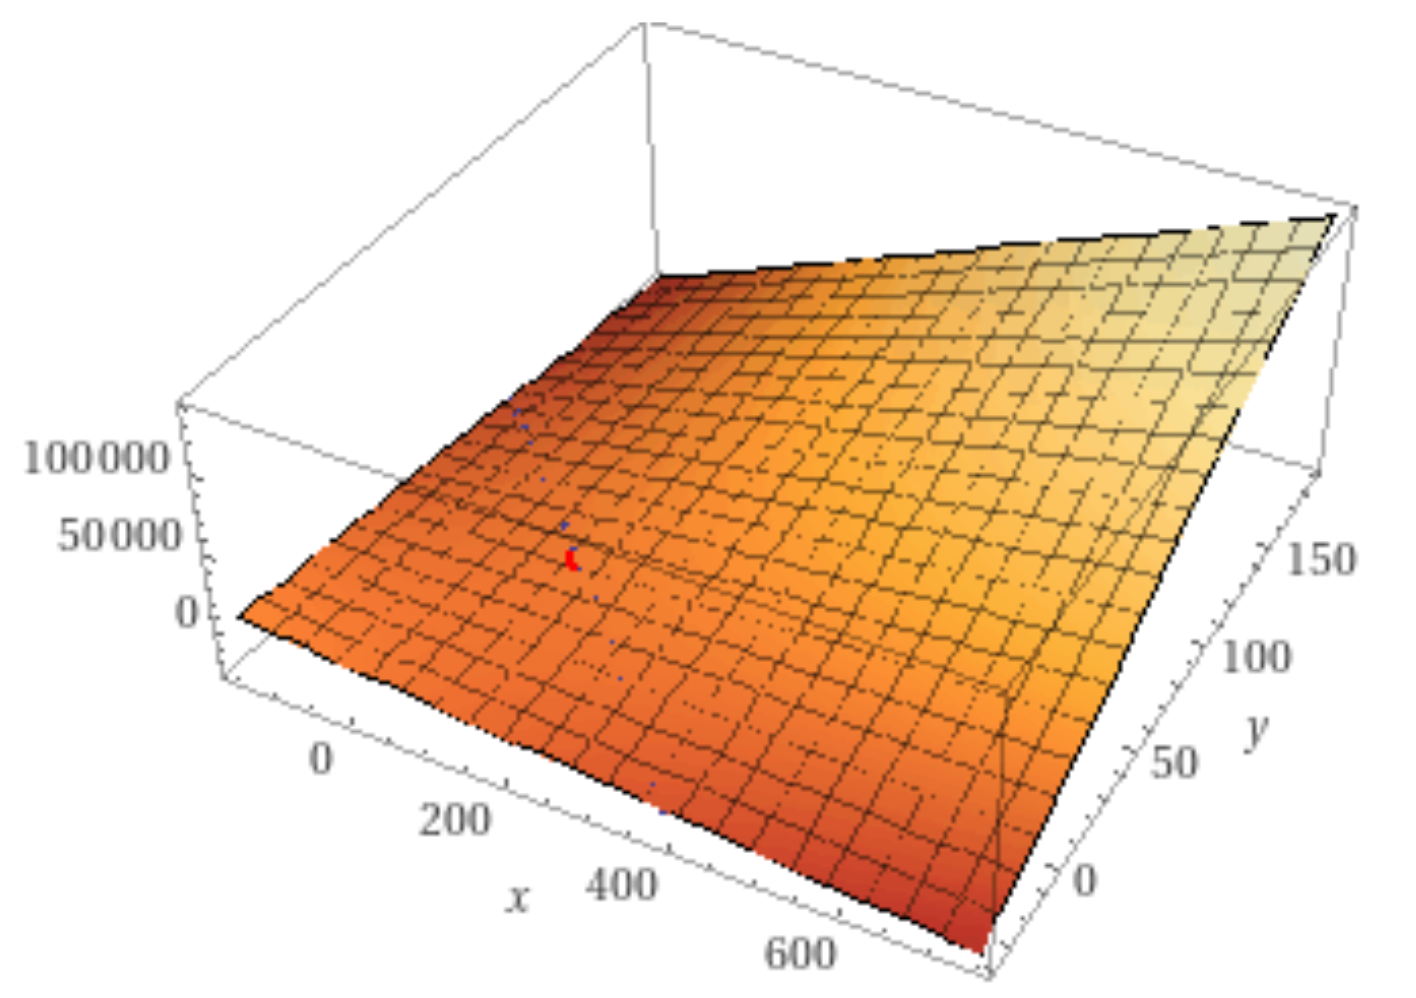
\includegraphics[width=0.4\textwidth]{prob1.png}
\hspace{1cm}
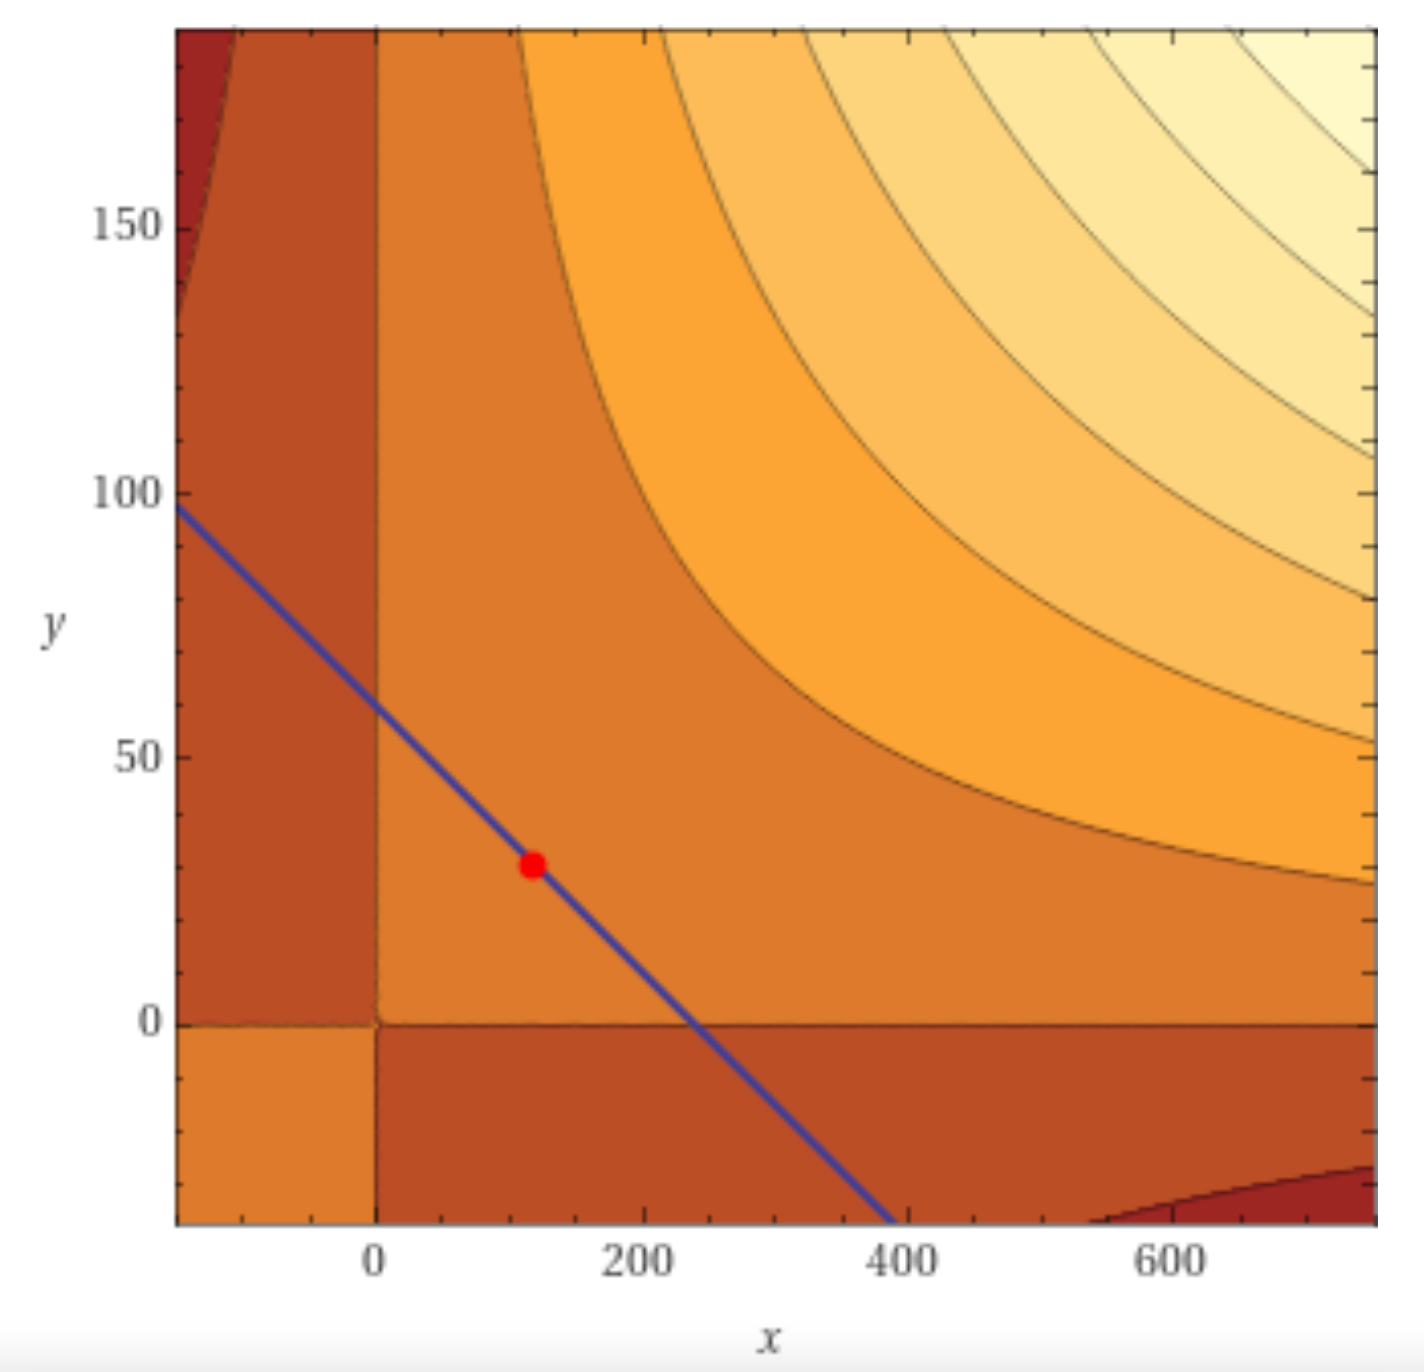
\includegraphics[width=0.4\textwidth]{prob2.png}
\end{frame}

\section{Analysis}

\subsection{User Requirements}

\begin{frame}
\frametitle{Analysis \\
\small \color{rwth-blue} User Requirements}
Users of the interface want to easily define and solve optimization problems with C++, including the ability to: 
\begin{itemize}
\item define (and modify) the objective function
\item define (and modify) the constraints
\item find the minima/maxima of the objective function regarding the constraints without having to write code to find the derivative
\end{itemize}

\end{frame}

\subsection{Use Case}

\begin{frame}
\frametitle{Analysis \\
\small \color{rwth-blue} Use Case}
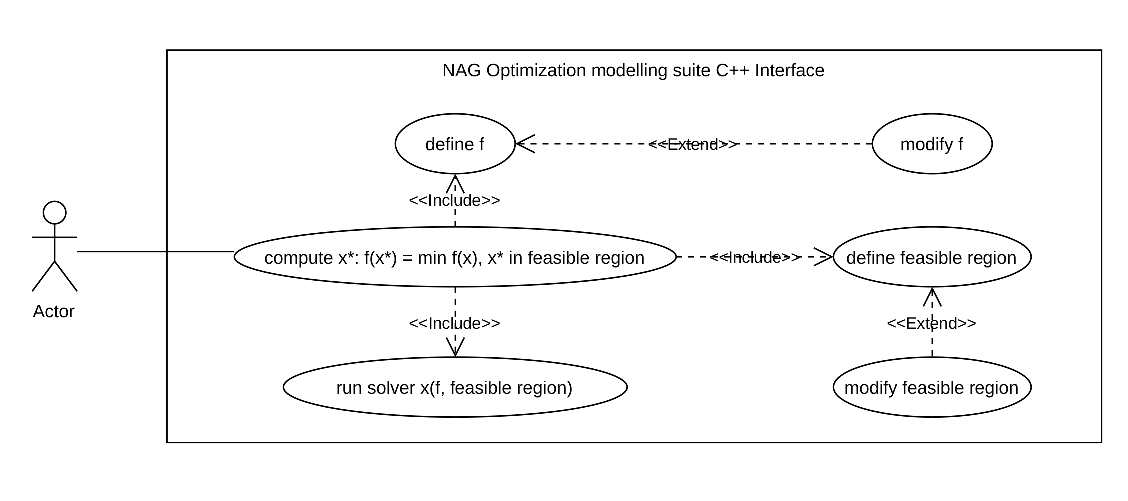
\includegraphics[width=\textwidth]{use case.pdf}
\end{frame}


\subsection{Essential Technical Background}

\begin{frame}
\frametitle{Analysis \\
\small \color{rwth-blue} Essential Technical Background}
\begin{itemize}
\item The NAG Library is a comprehensive collection of routines for the solution of numerical and statistical problems, comparable to FICO Xpress or Gurobi.
\item The NAG Optimization modelling suite is a part of the NAG Library, and is a suite of routines which allows the user to define and solve various optimization problems in a uniform manner.
\end{itemize}
\vspace{1em}
\begin{figure}
	
\includegraphics[width=4cm]{naglogo.png}
\end{figure}
\end{frame}


\begin{frame}
\frametitle{Analysis \\
\small \color{rwth-blue} Essential Technical Background}
\textbf{Optimization problem is defined as: }
$${\displaystyle {\begin{aligned}
&{\operatorname{minimize}} &&f(x)\\ &{\operatorname{subject\; to}}&& \mathit x \in \mathit{F}\end{aligned}}}$$ 
where x denotes the decision variables, f(x) the objective function and \textit{F} the feasibility set. We assume that $\mathit{F} \subset \mathbb{R}^n$. 

\end{frame}

\begin{frame}
\frametitle{Analysis \\
\small \color{rwth-blue} Essential Technical Background}
\textbf{Optimization problem classification:}\\ \vspace{2ex}
1. Type of objective function:
	\begin{itemize}
	\item Linear: ${\displaystyle f(x) = c^T x + c_0 , c  \in \mathbb{R}^n}$
	\item Non-linear: e.g. ${\displaystyle f(x)=(1-{x_1})^2+100 \cdot ({x_2}-{x_1}^2)^2}$
	\end{itemize}
\vspace{1em}
2. Type of constraints: 
	\begin{itemize}
	\item Unconstrained
	\item Simple bound: ${\displaystyle l_x \leq x \leq u_x}$, ${\displaystyle l_x }$ and ${\displaystyle u_x}$ are n-dimensional vectors.
	\item Linear constraint: ${\displaystyle l_B \leq B_x \leq u_B}$, B is a general ${\displaystyle m_B}$ x n rectangular matrix and ${\displaystyle l_x }$ and ${\displaystyle u_x}$ are n-dimensional vectors.
	\item Non-linear constraint: ${\displaystyle  l_g \leq g(x) \leq u_g}$
	\item and more...
	\end{itemize}
\end{frame}

\begin{frame}
\frametitle{Analysis \\
\small \color{rwth-blue} Essential Technical Background}
\vspace{1ex}
\textbf{These combinations define specific optimization problems:}\\
\begin{enumerate}
\item Linear programming problem: linear objective function, linear constraints and simple bounds.
$${\displaystyle {\begin{aligned}
&{\underset{x\in \mathbb{R}^n}{\operatorname{minimize}} }&&c^Tx\\&{\operatorname{subject\; to}}&& l_B \leq Bx \leq u_B,\\&&&l_x \leq x \leq u_x.\end{aligned}}}$$ 
\item Nonlinear programming problem: general nonlinear objective function and any of the nonlinear, quadratic, linear or bound constraints.
$${\displaystyle {\begin{aligned}
&{\underset{x\in \mathbb{R}^n}{\operatorname{minimize}} }&&f(x)\\ &{\operatorname{subject\; to}}&& l_g \leq g(x) \leq u_g,\\&&&l_B \leq Bx \leq u_B,\\&&&l_x \leq x \leq u_x.\end{aligned}}}$$ 
\end{enumerate}
A lot more: Quadratically Constrained Quadratic Programming, Least Squares, Data Fitting...But we focus on these two for the project.
\end{frame}

\begin{frame}
\frametitle{Analysis \\
\small \color{rwth-blue} Essential Technical Background}
\large\underline{\textbf{dco/c++:}} 
\vspace{1em}
\begin{itemize}
	\item An AD software tool for computing sensitivities of C++ codes
\end{itemize}
\end{frame}

\begin{frame}
\frametitle{Analysis \\
\small \color{rwth-blue} Essential Technical Background -- Interface layering}
\begin{itemize}
	\item The NAG library (specifically the optimization modelling suite) is available in several languages, including Fortran, C, and an experimental C++ interface that is hard to use.
	\item A C++ layer is to be built on top of the given C++ interface, allowing the user to access the library by writing easier code. The C++ interface also utillizes dco/c++ for addition functions not existing in the given version.
\end{itemize}
\centering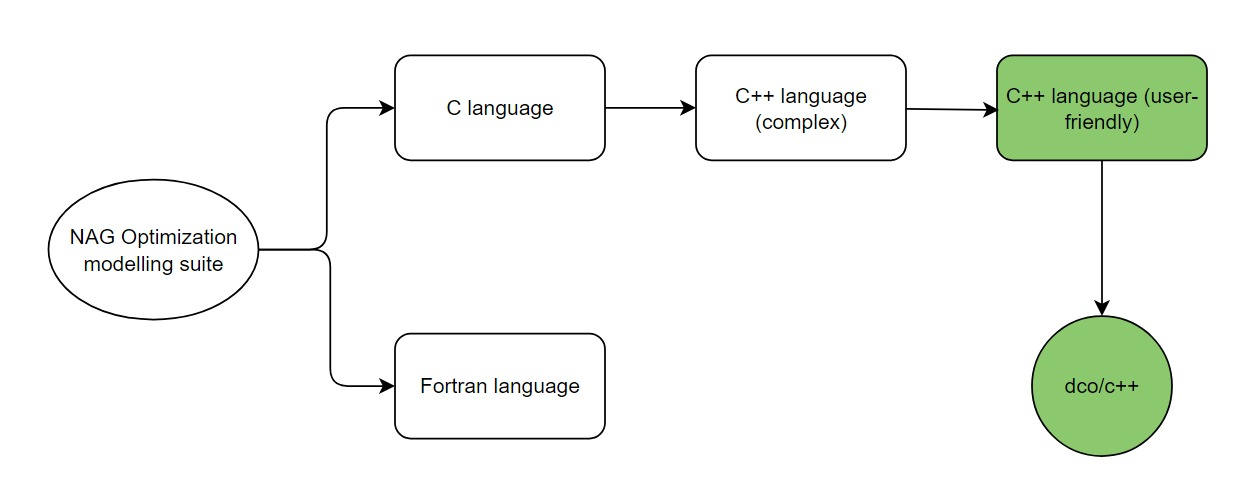
\includegraphics[width=4in]{layering.jpeg}
\end{frame}

\subsection{System Requirements}

\begin{frame}
\frametitle{Analysis \\
\small \color{rwth-blue} System Requirements}

Functional:
\begin{itemize}
\item defining optimization problems, including:
	\begin{itemize}
	\item the ability to define and modify objective functions
	\end{itemize}
\item automatic computation of derivatives
\item recognisation of linear contraints
	\begin{itemize}
	\item automatic modification of problem to reflect linearity
	\end{itemize}
\item solve problems with either automatic solver choice or manual choice from the 3 solvers: e04mt, e04kf, e04st
\end{itemize}
Nonfunctional:
\begin{itemize}
\item backend: NAG Optimization Modelling Suite, C++ interface
\item interface implementation in C++ using OOP
\item testing with CTest and googletest
\item documentation with doxygen
\item automatic computation of derivatives and recognisation of linear contraints with dco/c++
\end{itemize}
\end{frame}


\section{Design}

\subsection{Class Candidates}
\begin{frame}
\frametitle{Design \\
\small \color{rwth-blue} Class Candidates}
\small How the pre-existing C++ interface works:
\small\begin{itemize}
	\item Uses a single class called “handle”, which contains everything: solver’s parameters (accuracy, monitoring, etc.) and problem definition (objective function, bounds) and more.
	\item No classes and class method, only functions.
	\item If a solver requires derivative of a function, the user must write it themselves, which is prone to errors.
\end{itemize}
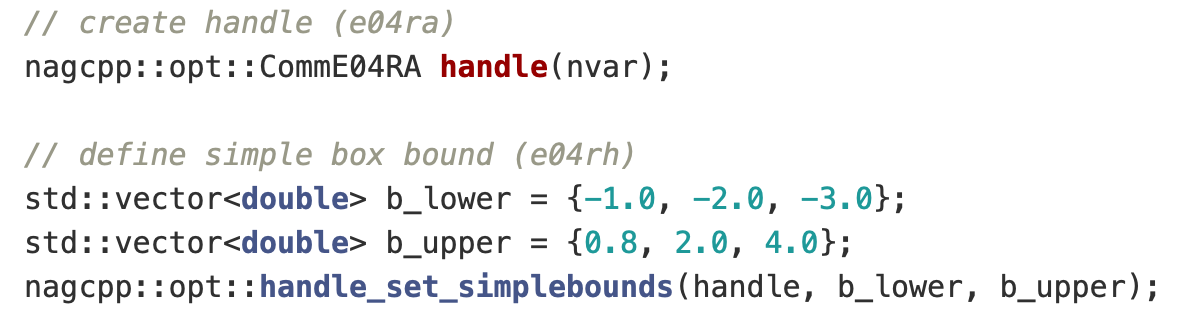
\includegraphics[width=0.5\textwidth]{preinterface1.png}
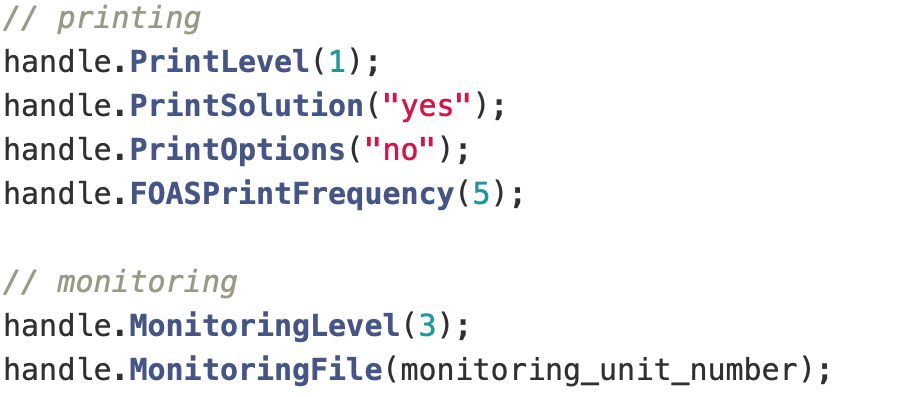
\includegraphics[width=0.35\textwidth]{preinterface2.png}
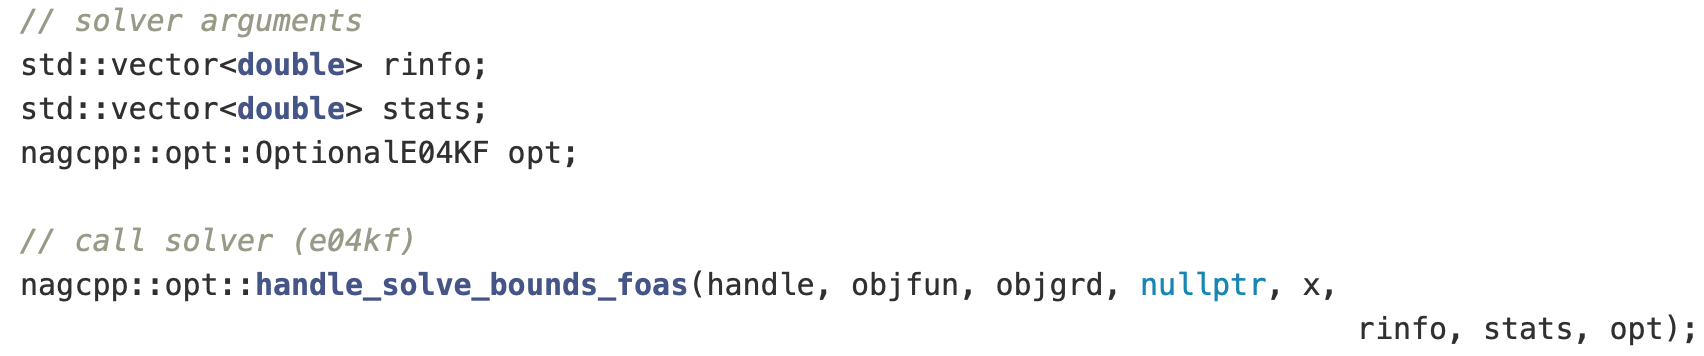
\includegraphics[width=0.8\textwidth]{preinterface3.png}
\end{frame}

\begin{frame}
\frametitle{Design \\
\small \color{rwth-blue} Class Candidates}
Some keywords/classes from the existing C++ interface which could be used as classes in ours:
\begin{itemize}
	\item problem
	\item solver
	\item dco/derivative
	\item bound
	\item function
		\begin{itemize}
			\item objectiveFunction
			\item constraintFunction
		\end{itemize}
	\item linearInfo
\end{itemize}
\end{frame}


\subsection{Class Model}

\begin{frame}
\frametitle{Design \\
\small \color{rwth-blue} Class Model}
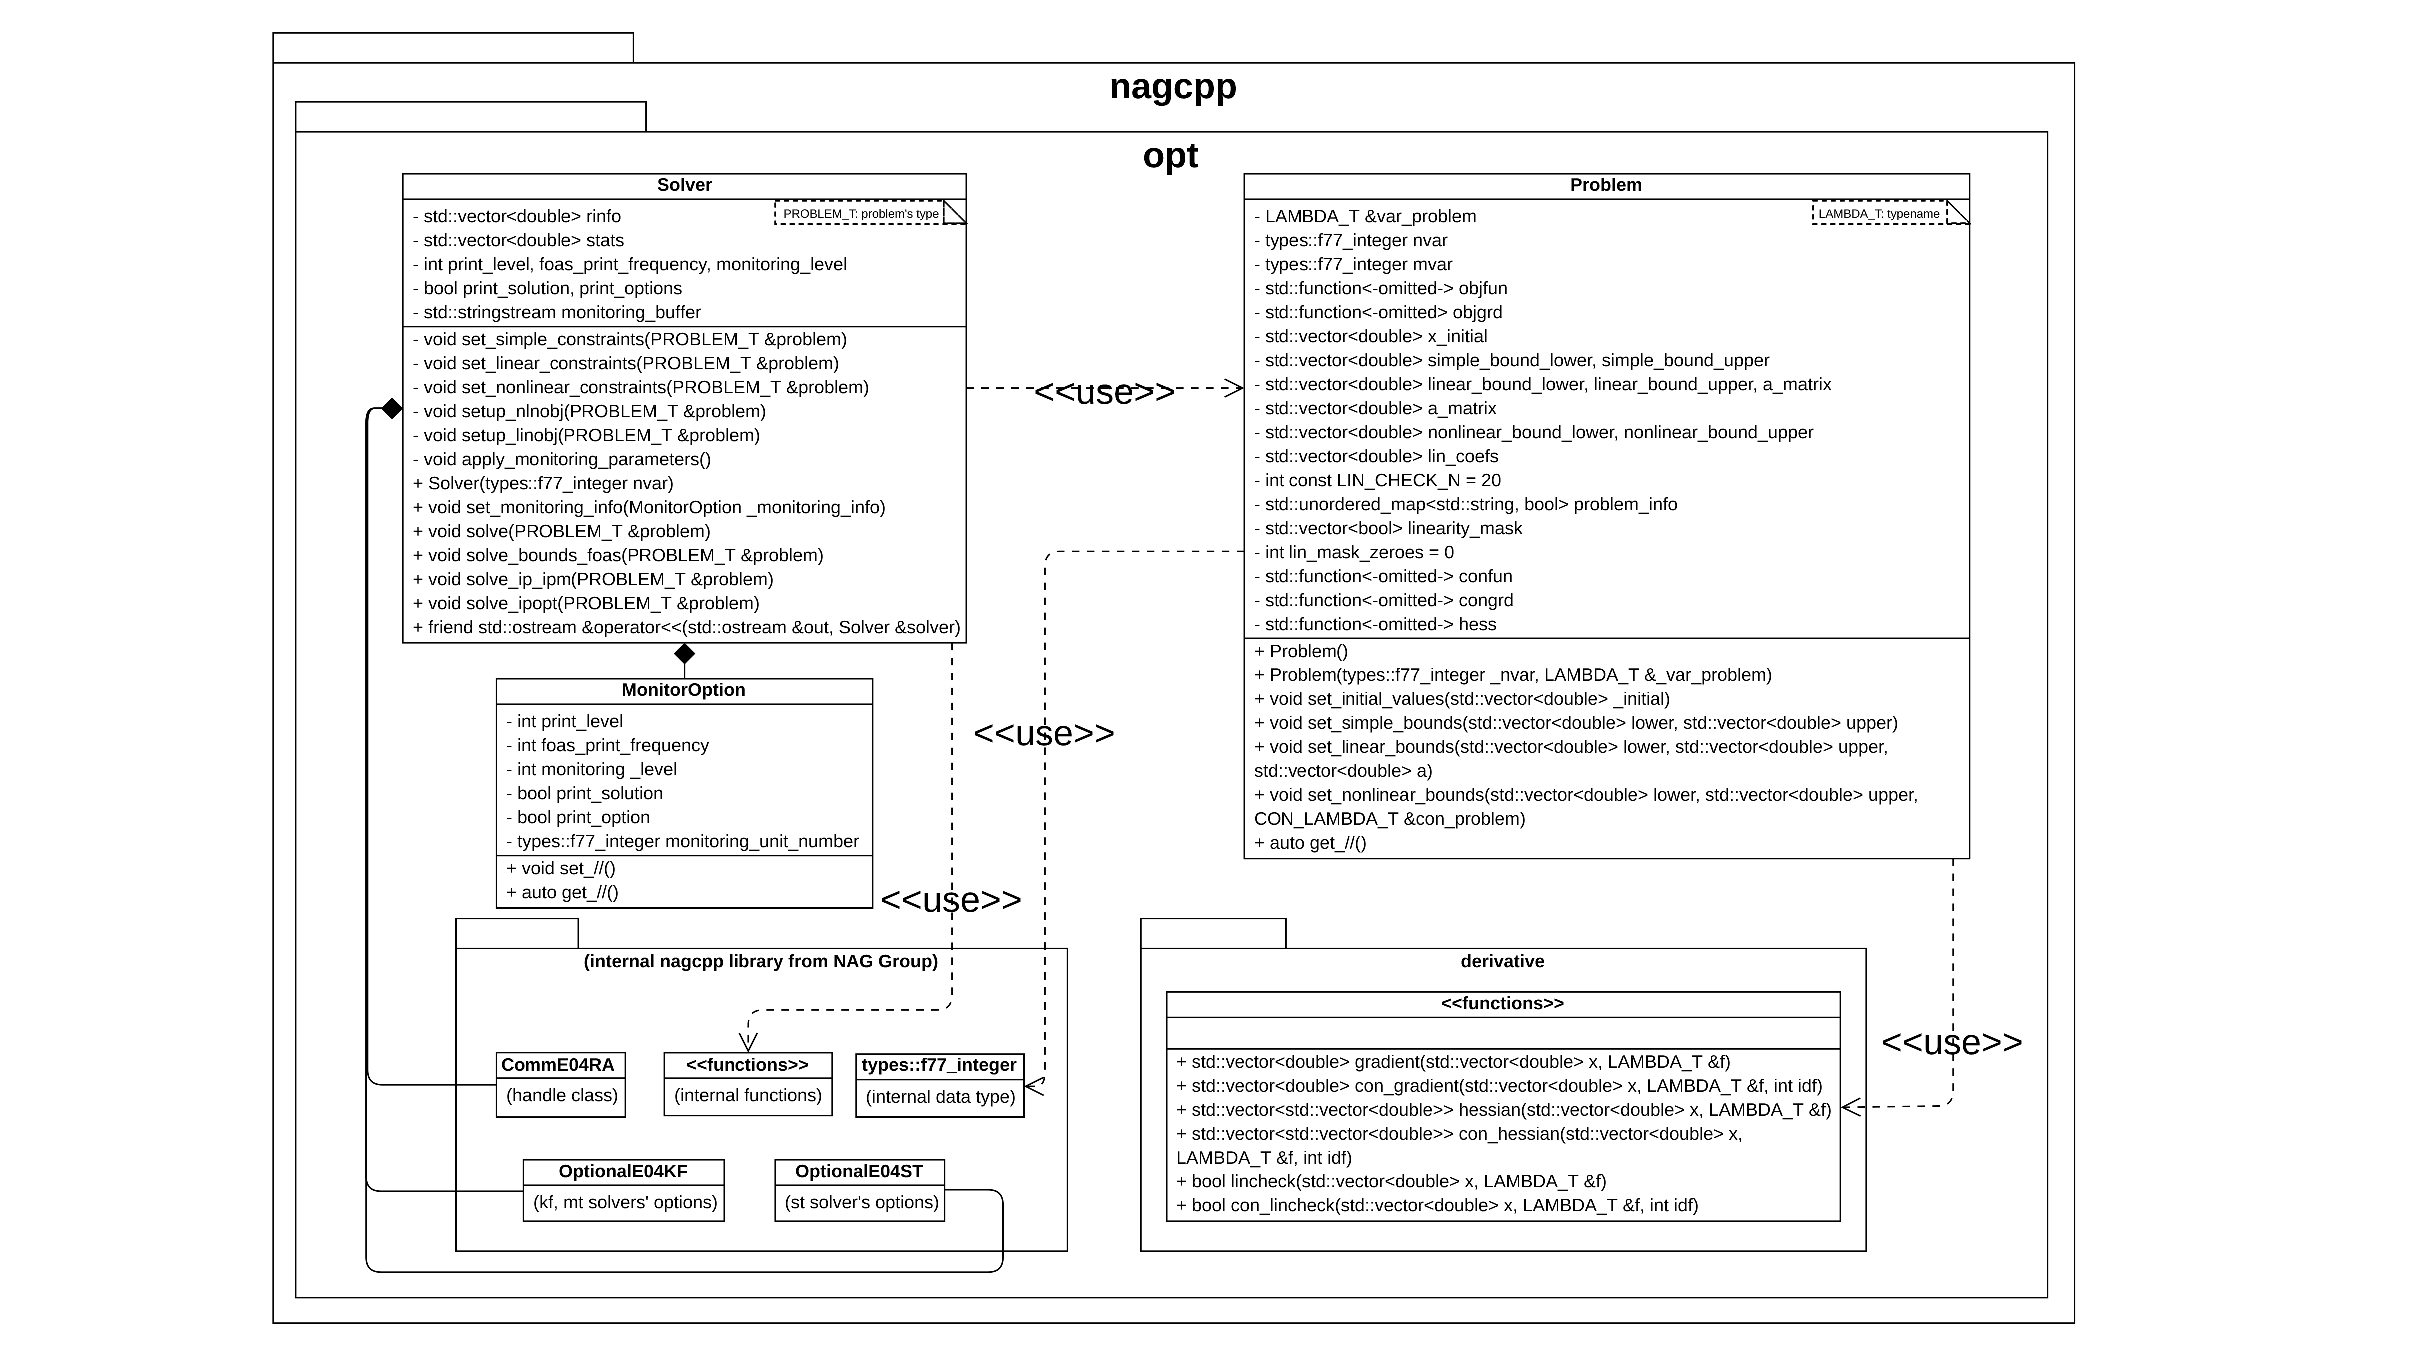
\includegraphics[height=0.95\textheight]{class diagram.pdf}
\end{frame}

\begin{frame}
\frametitle{Design \\
\small \color{rwth-blue} Class Model - Optimize function}
\centering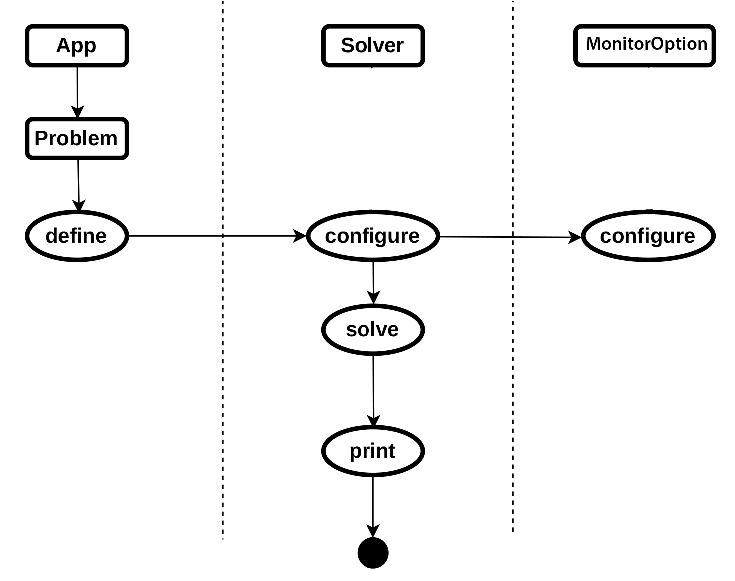
\includegraphics[height=0.95\textheight]{Class Model - Optimize function.pdf}
\end{frame}

\section{Implementation}

\subsection{Development Infrastructure}
\begin{frame}
\frametitle{Implementation \\
\small \color{rwth-blue} Development Infrastructure}
\begin{itemize}
	\item Target platform: Linux devices, specifically the Virtual Machine provided by Prof. Naumann
	\item Programming language: C++ 20
	\item Compiler: gcc
	\item Build system: CMake
	\item Runtime library: NAG Library with C++ interface, dco/c++, the standard ones (std, math.h, etc.)
\end{itemize}
\end{frame}

\subsection{Source Code}

\begin{frame}
\frametitle{Implementation \\
\small \color{rwth-blue} Source Code}
\vspace{1em}
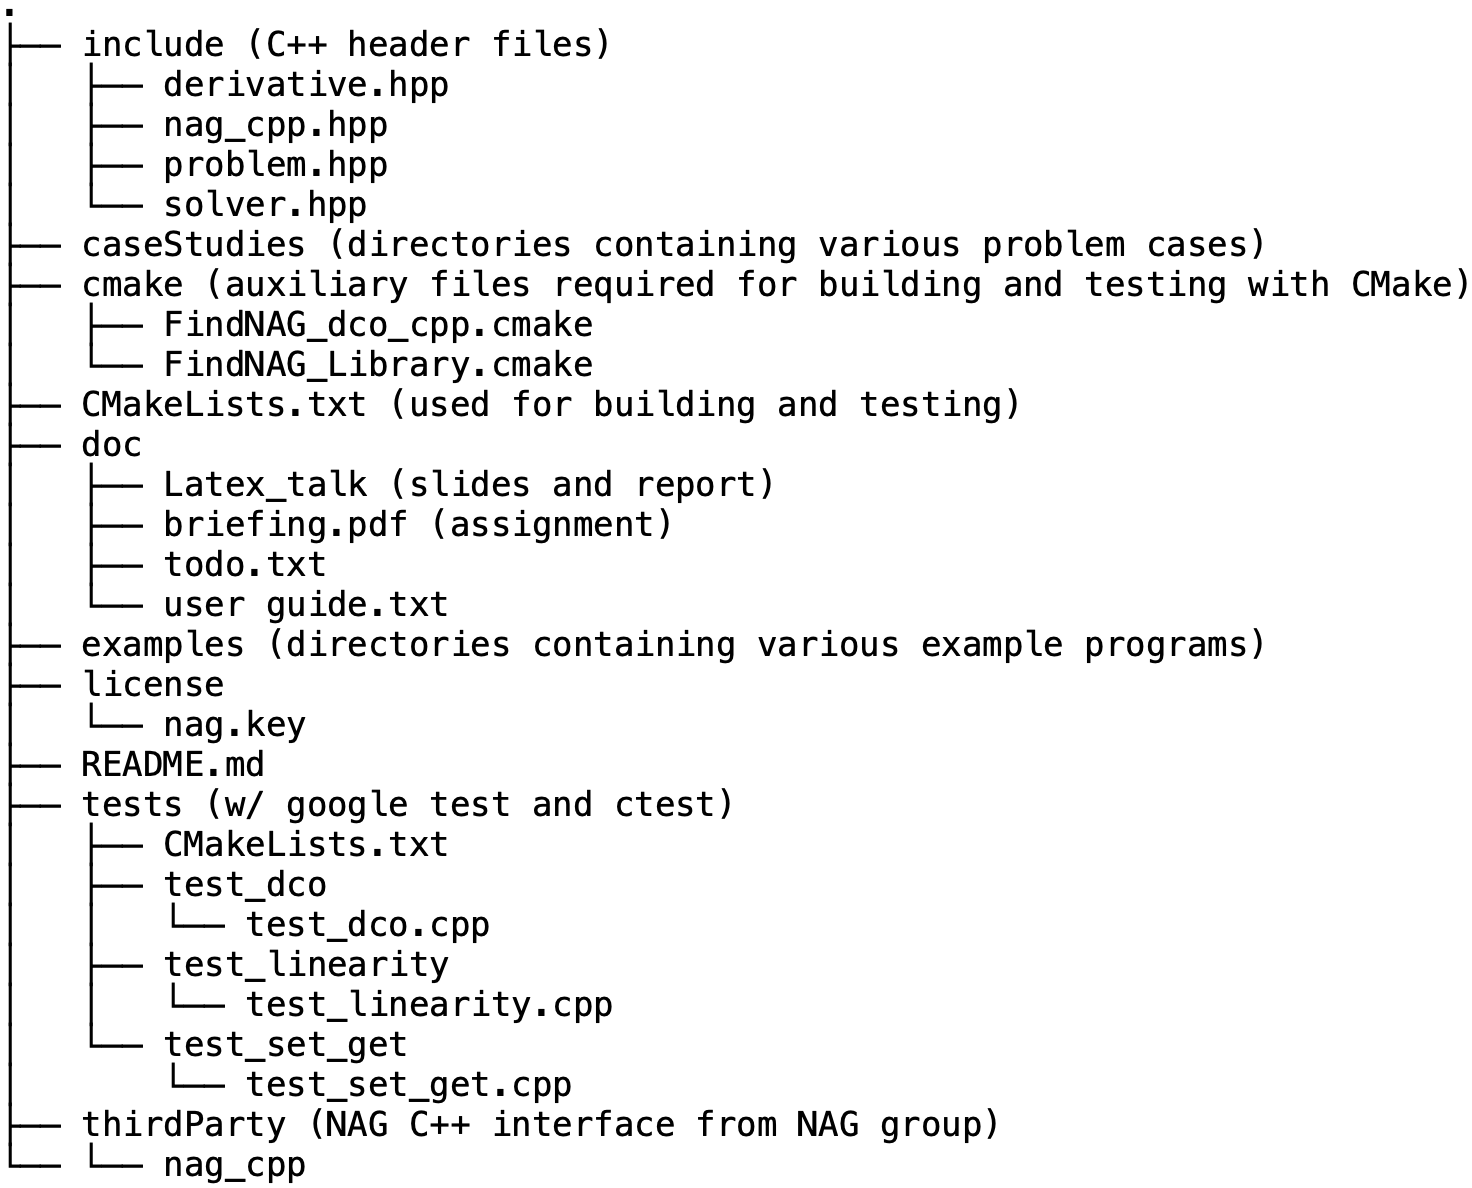
\includegraphics[height=\textheight]{tree.png}
\end{frame}


\begin{frame}
\frametitle{Implementation \\
\small \color{rwth-blue} Source Code}
\textbf{problem.hpp:}\\ \vspace{1em}
1. contains the objective functions, constraint functions and various kinds of bounds\\
\vspace{1em}
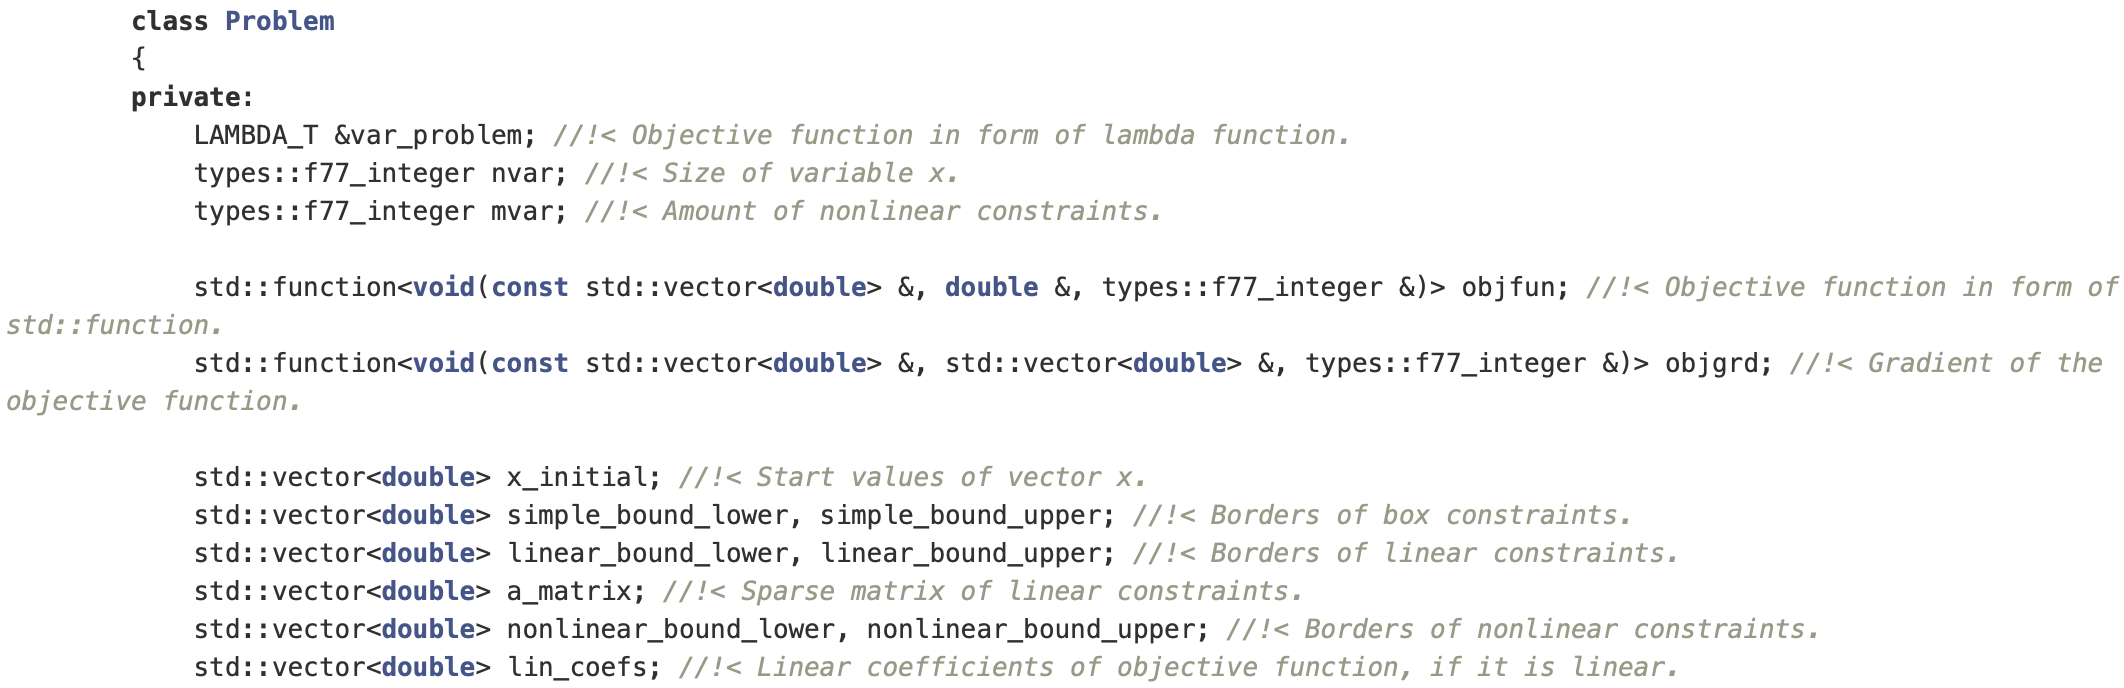
\includegraphics[width=\textwidth]{code_problem1.png}
\end{frame}

\begin{frame}
\frametitle{Implementation \\
\small \color{rwth-blue} Source Code}
2. contains the set\_//\_() functions\\
\vspace{1em}
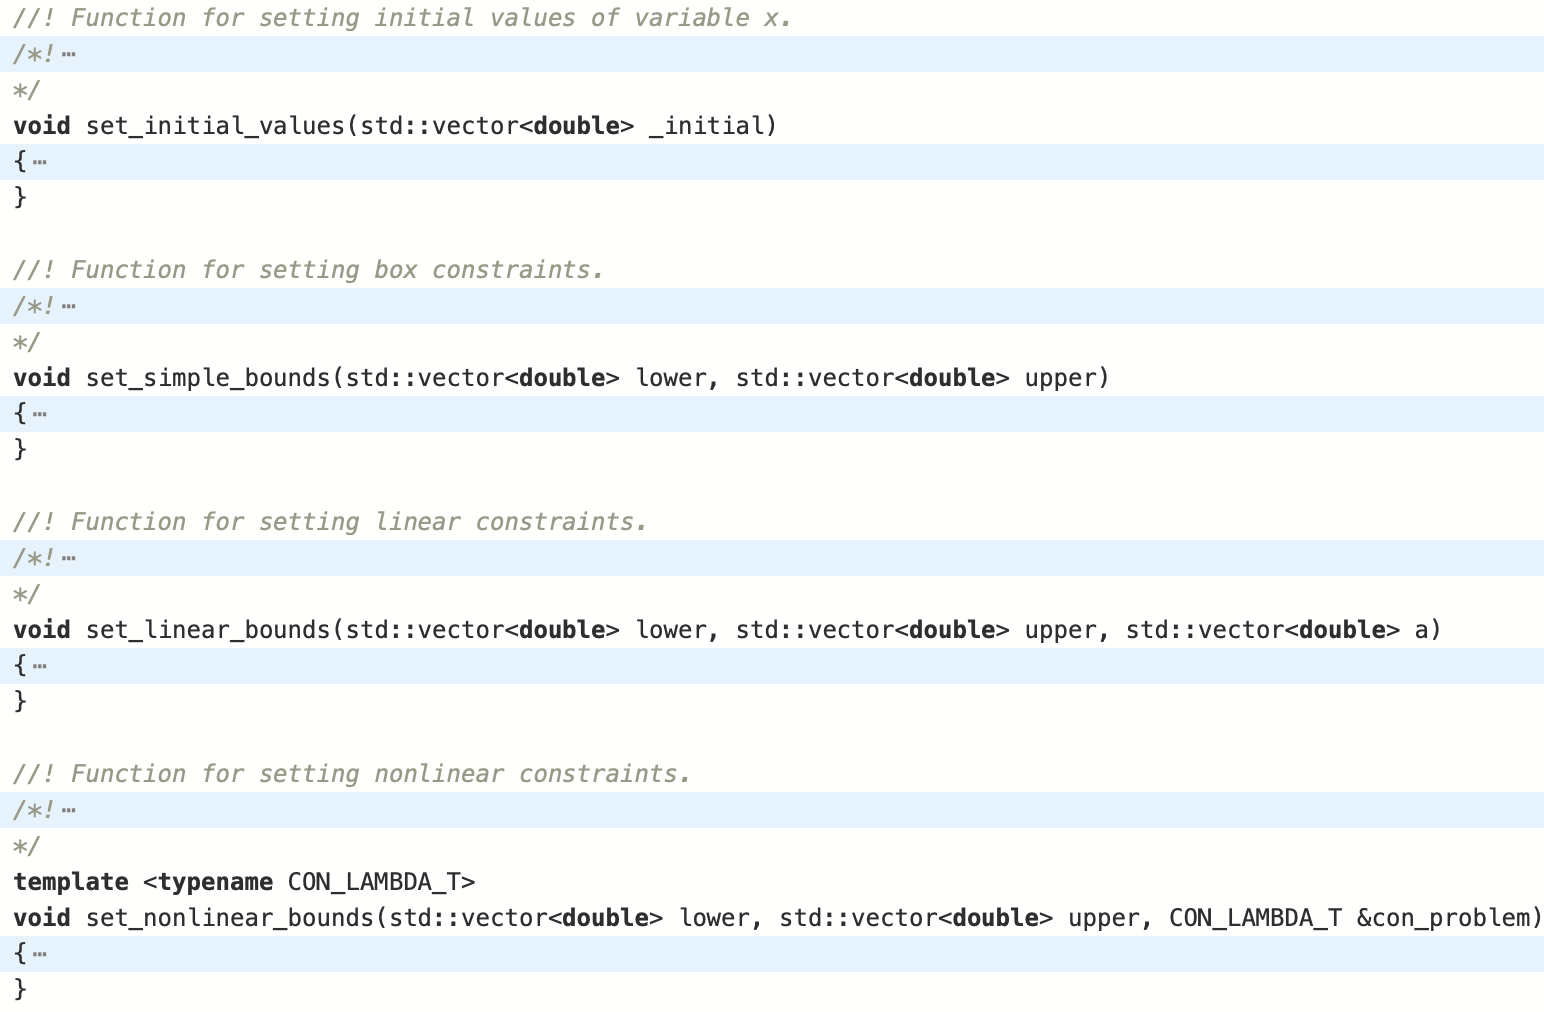
\includegraphics[width=0.8\textwidth]{code_problem2.png}
\end{frame}

\begin{frame}
\frametitle{Implementation \\
\small \color{rwth-blue}Source Code}
3. set\_nonlinear\_bounds() detects whether bounds are non-linear or not and sets them accordingly\\
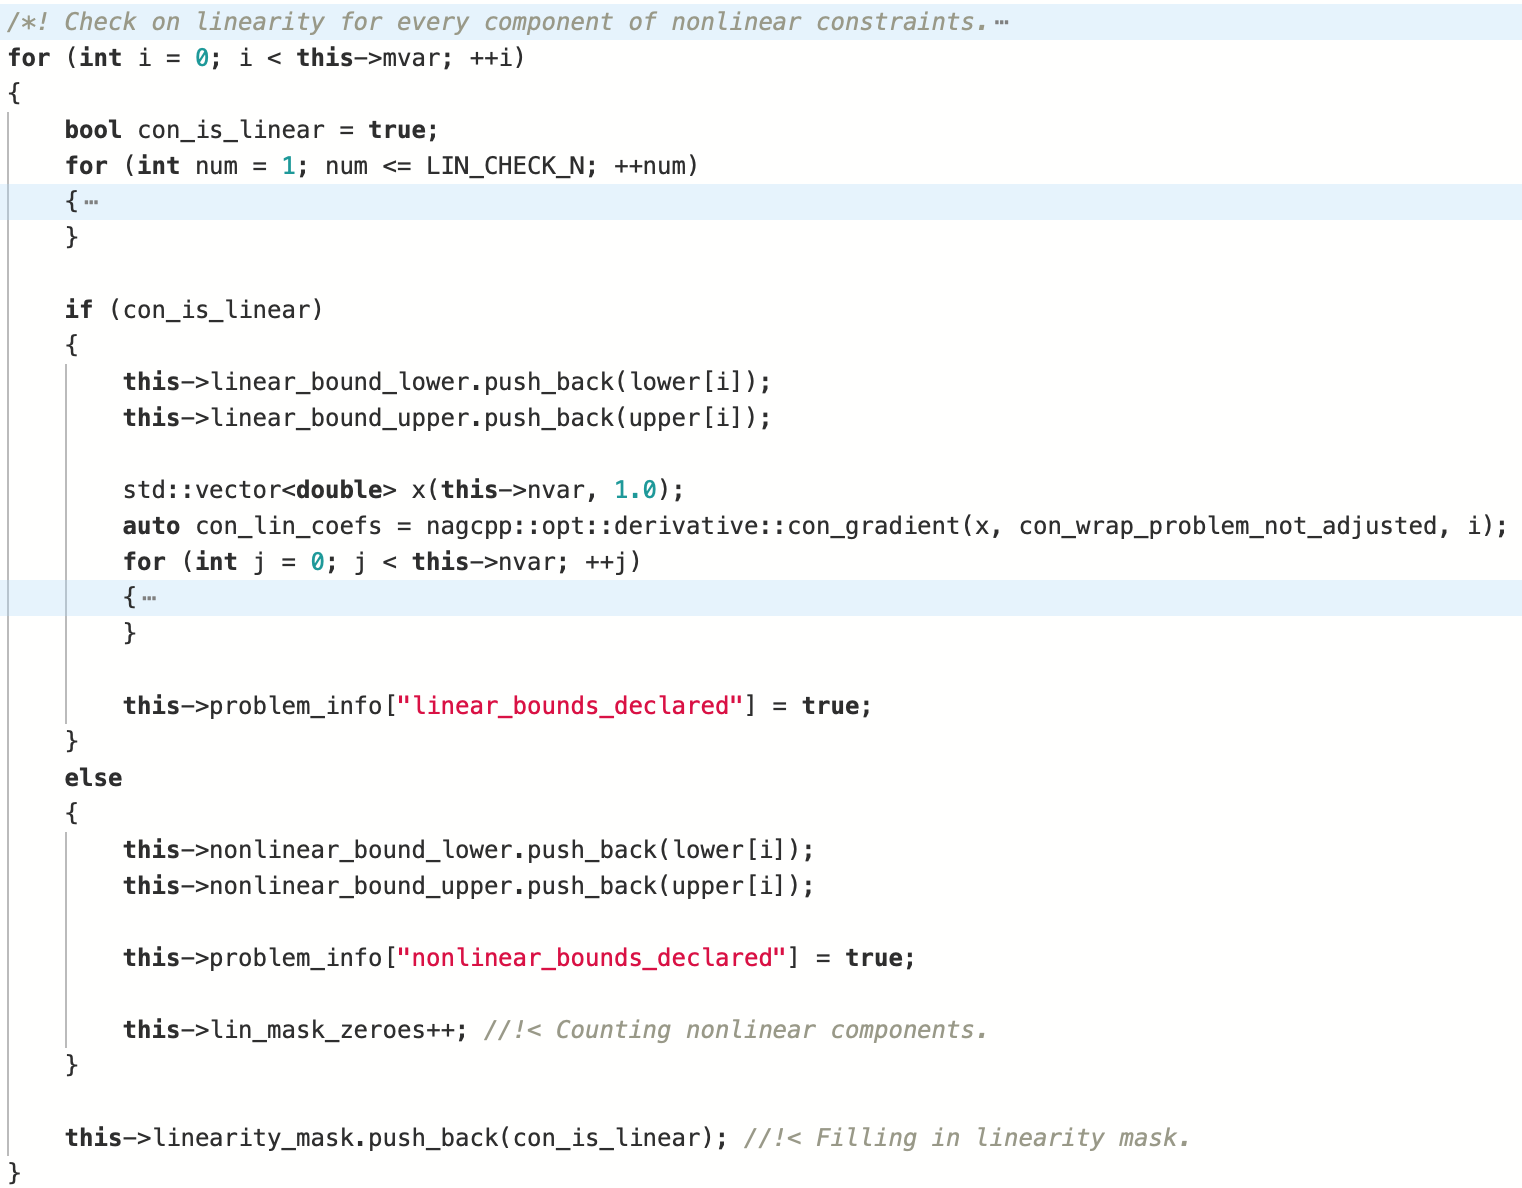
\includegraphics[width=0.75\textwidth]{code_problem3.png}
\end{frame}

\begin{frame}
\frametitle{Implementation \\
\small \color{rwth-blue} Source Code}
\textbf{derivative.hpp:}\\ \vspace{1ex}
\begin{itemize}
	\item uses dco/c++
	\item checks linearity by examining whether the derivative is zero or not
\end{itemize}
\vspace{1em}
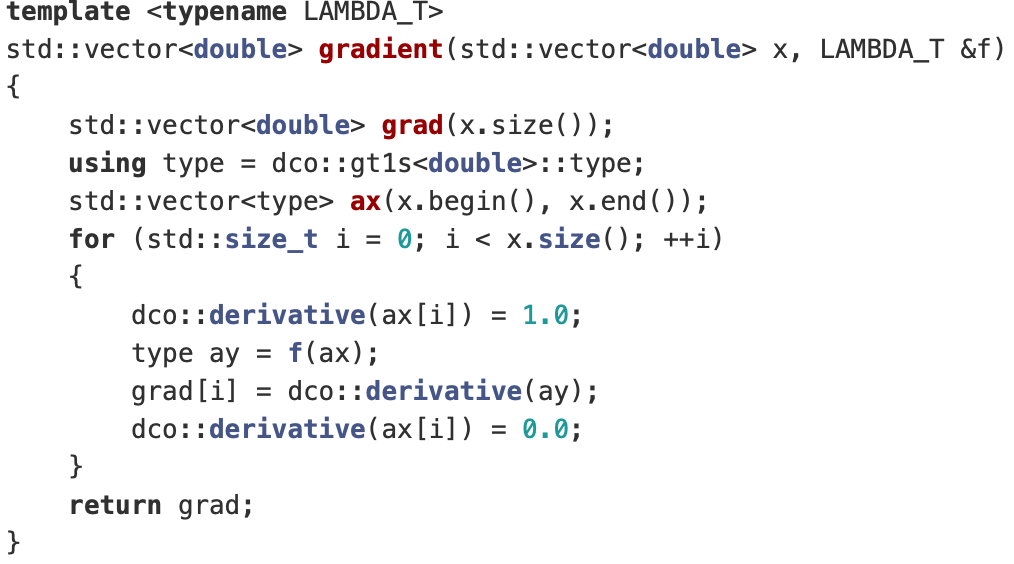
\includegraphics[width=0.8\textwidth]{code_derivative.png}
\end{frame}

\begin{frame}
\frametitle{Implementation \\
\small \color{rwth-blue} Source Code}
\textbf{monitor.hpp:}\\ \vspace{1ex}
MonitorOption: a simple class used to hold monitoring options\\
\vspace{1em}
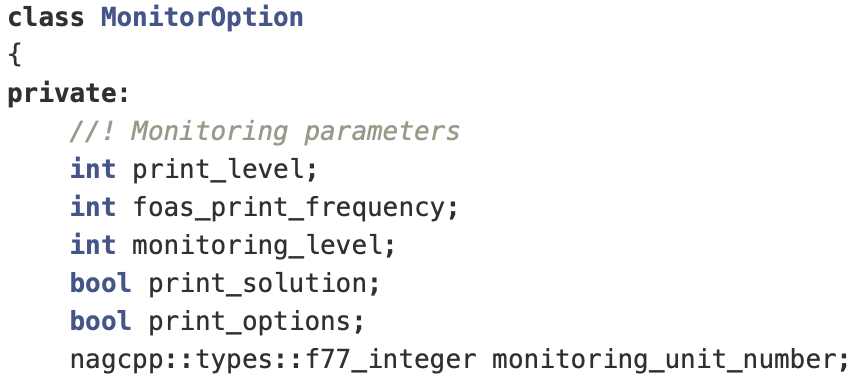
\includegraphics[width=0.8\textwidth]{code_monitor.png}
\end{frame}

\begin{frame}
\frametitle{Implementation \\
\small \color{rwth-blue} Source Code}
\vspace{1ex}
\textbf{solver.hpp:}\\ \vspace{1ex}
1. contains CommE04RA handle, the internal NAG C++ interface’s communicator class, as well as solver’s options\\
2. contains set\_//() wrapper functions to pass problem definition into the handle\\
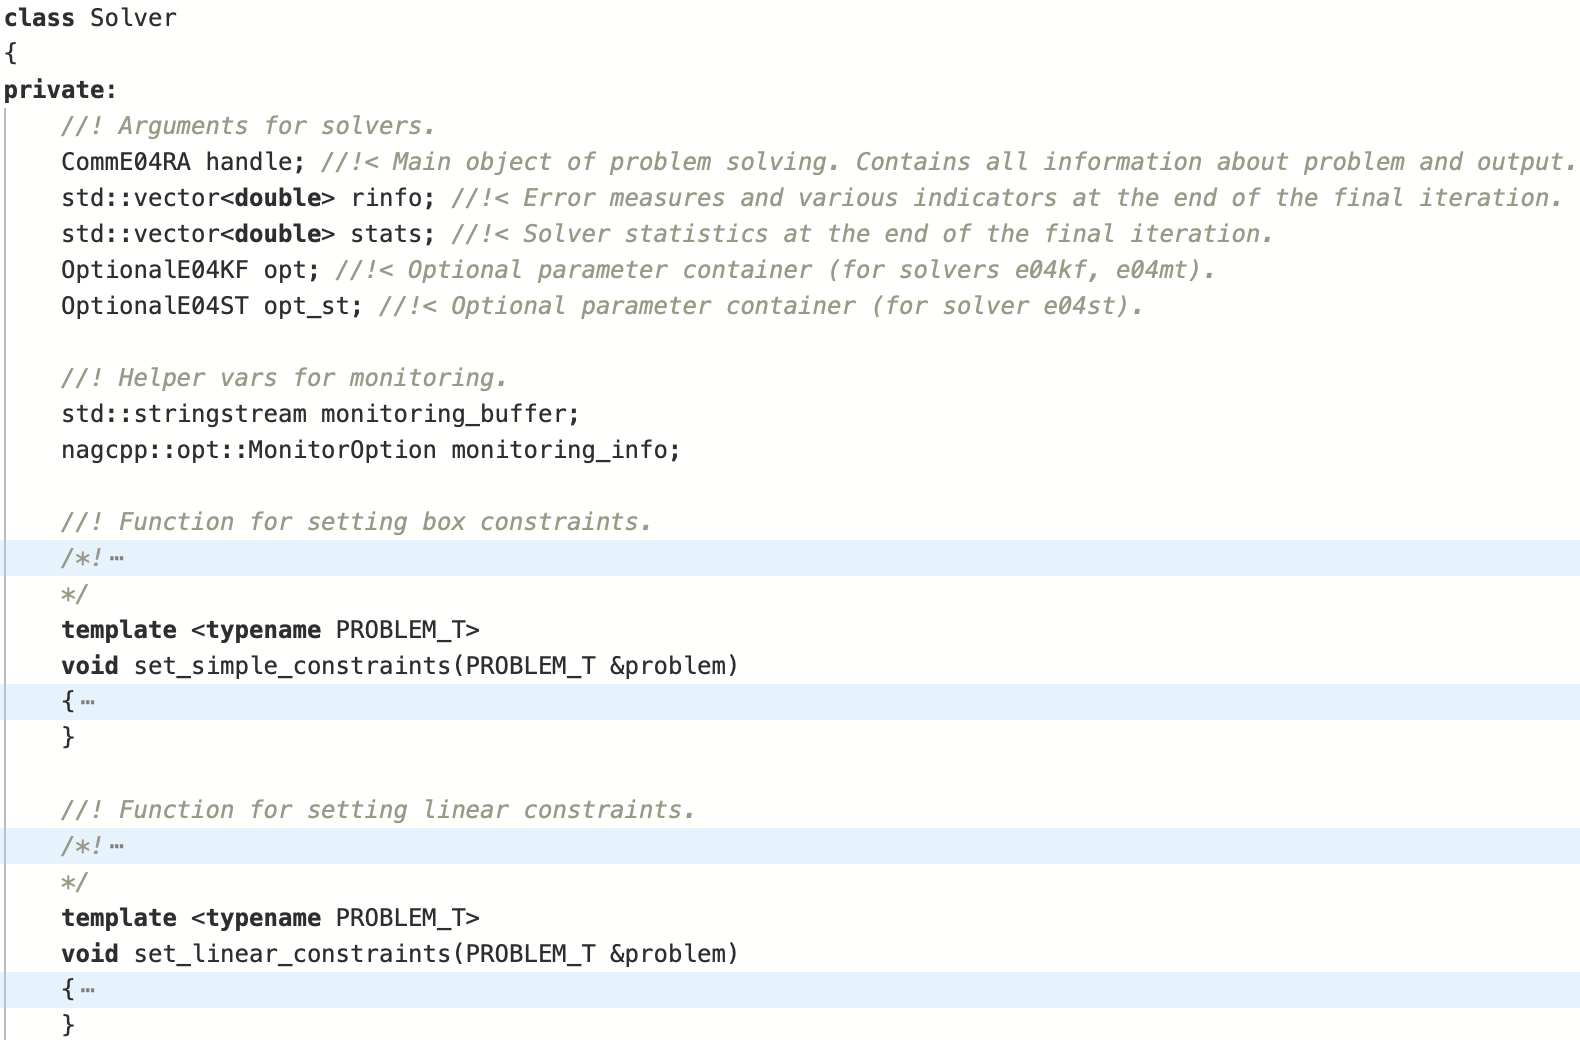
\includegraphics[width=0.75\textwidth]{code_solver1.png}
\end{frame}

\begin{frame}
\frametitle{Implementation \\
\small \color{rwth-blue} Source Code}
3. solve() automatically chooses from one of the 3 solvers: e04kf, e04mt, and e04st which is based on the problem’s type of constraints and their linearity.\\
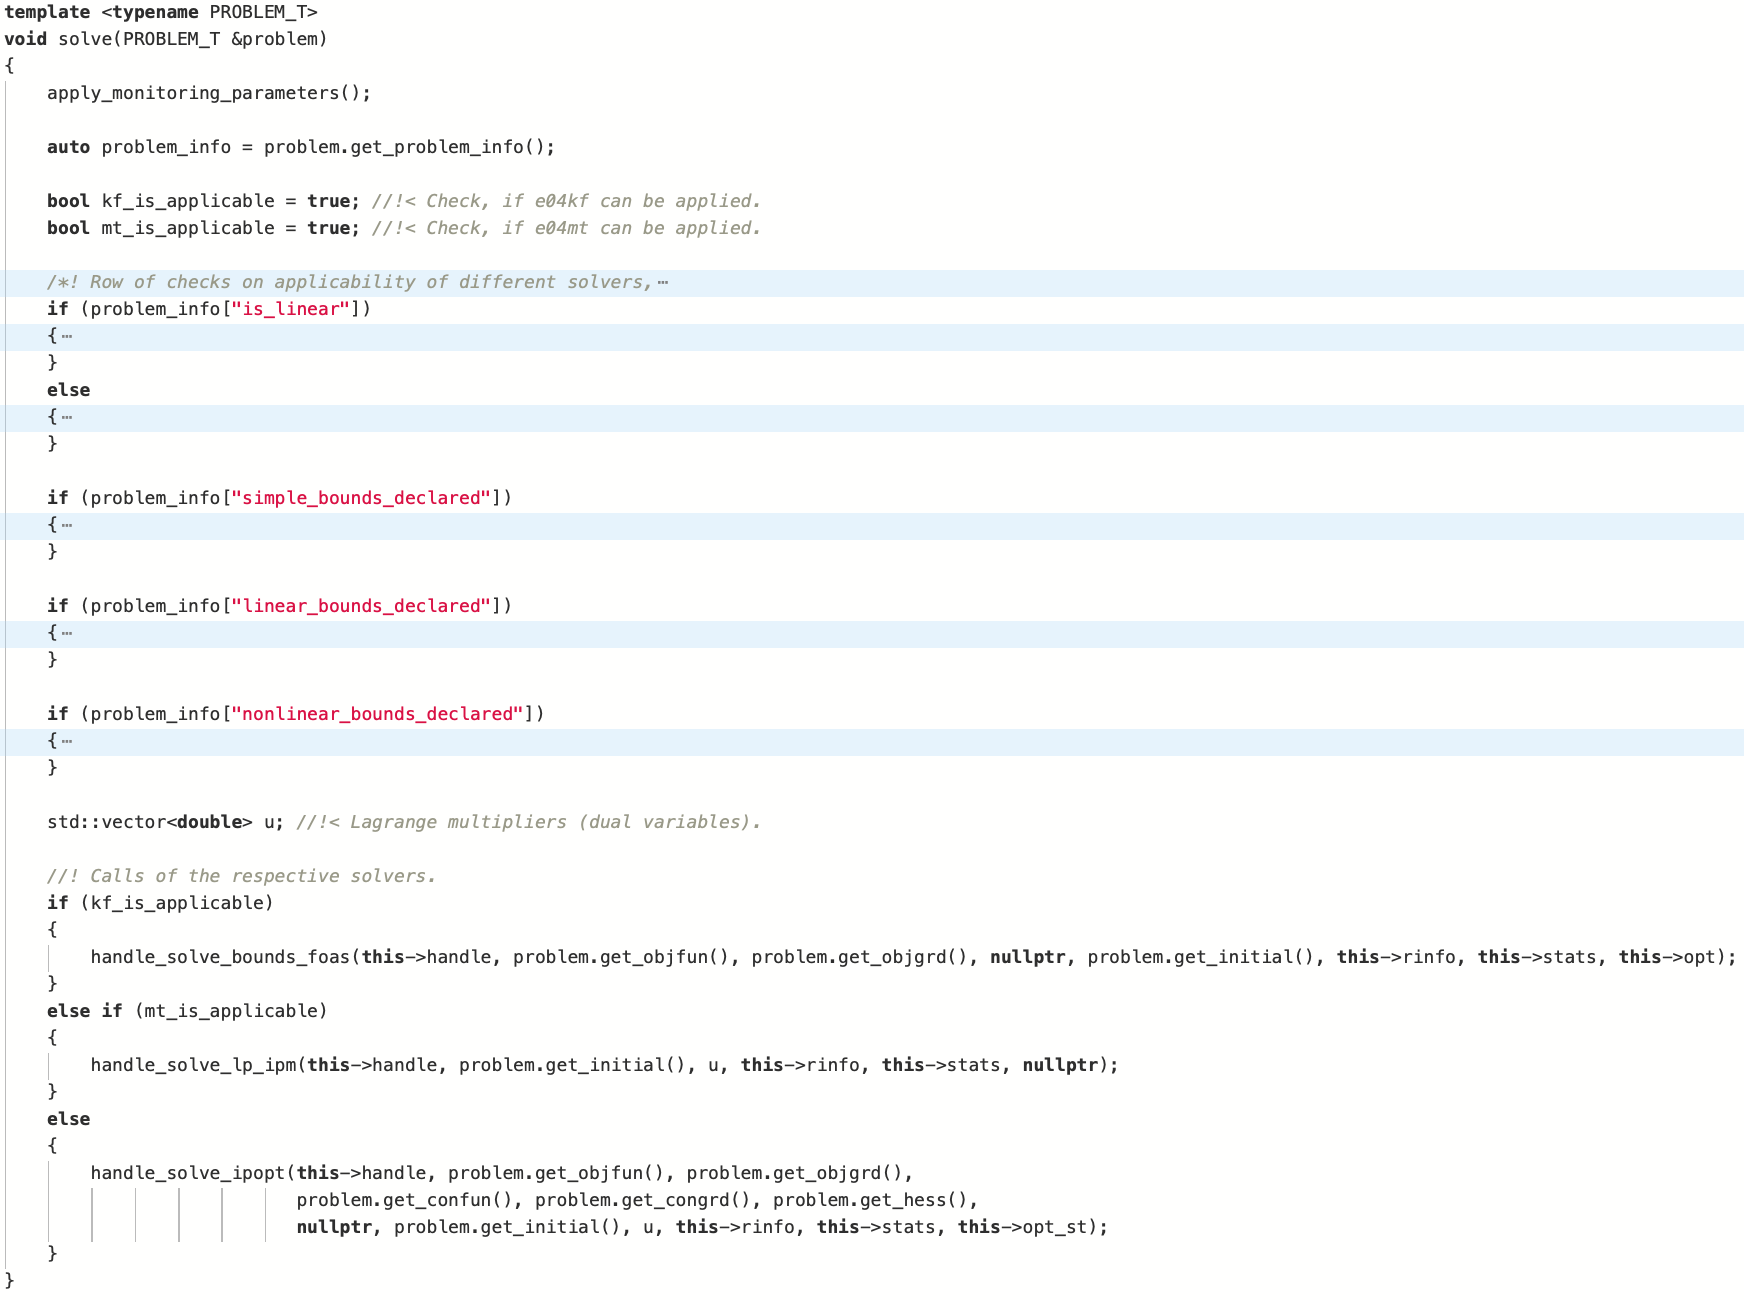
\includegraphics[width=0.75\textwidth]{code_solver2.png}
\end{frame}

\begin{frame}
\frametitle{Implementation \\
\small \color{rwth-blue} Source Code}
\textbf{Documentation:}\\ \vspace{1ex}
Every function and its parameters are documented thoroughly.\\
\vspace{1em}
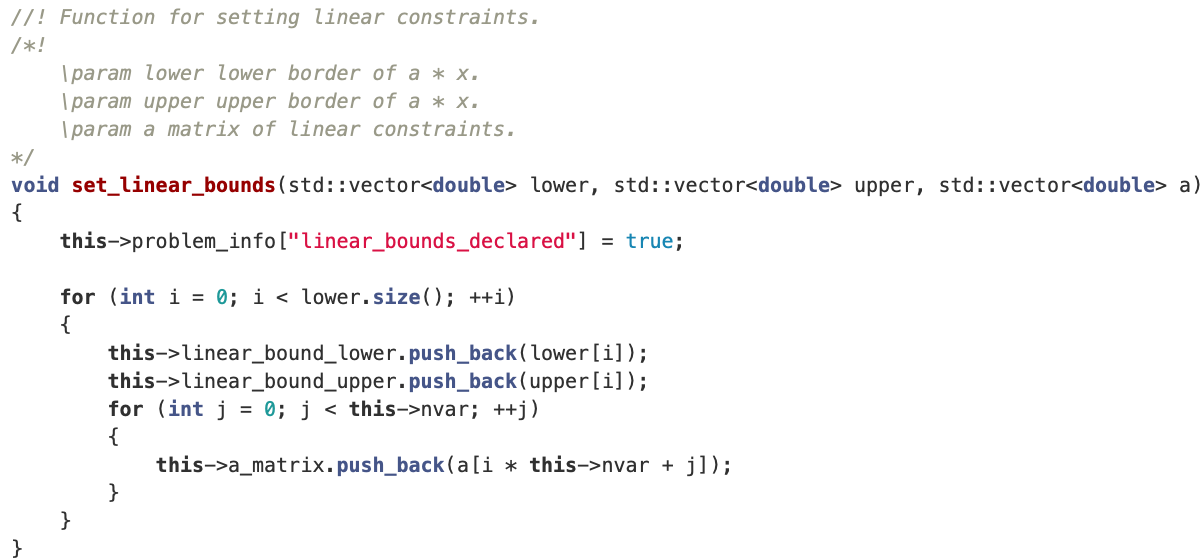
\includegraphics[width=0.9\textwidth]{code_docu.png}
\end{frame}

\begin{frame}
\frametitle{Implementation \\
\small \color{rwth-blue} Source Code}
\textbf{Example of a simple program by the user:}\\ \vspace{1em}
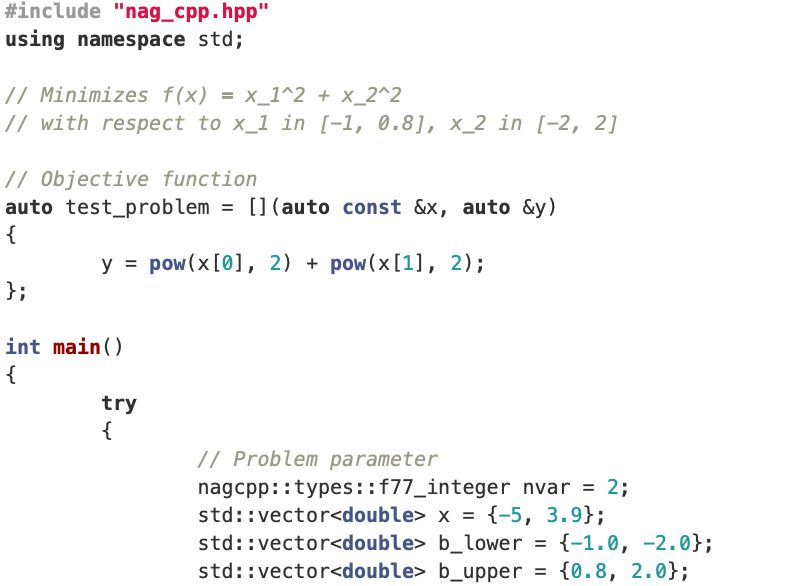
\includegraphics[width=0.47\textwidth]{code_eg1.png}
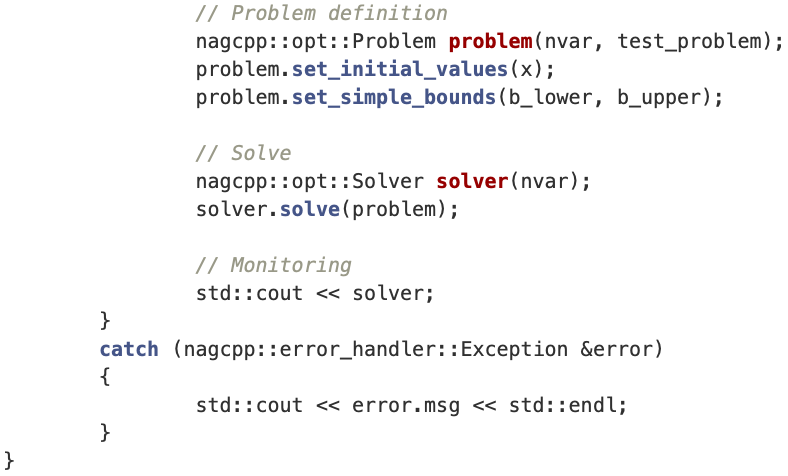
\includegraphics[width=0.47\textwidth]{code_eg2.png}
\end{frame}

\begin{frame}
\frametitle{Implementation \\
\small \color{rwth-blue} Discussion of Source Code}
\begin{itemize}
	\item Focus on clean, readable, and well documented C++ code without memory leaks or invalid memory access (tested with Valgrind).
	\item Modern C++ features are used, such as class template type deduction via construction from 2017.
	\item Mathematically less complex for the user than the existing interface – automatic derivation, no worry about sparse matrix by e04mt, etc. 
	\item The whole point is to be user-friendly. The previous example program written with the original interface was approx. 90 lines of code, which is now 40.
	\item In total we wrote 1400+ lines of code, most of it in \texttt{problem.hpp}.
	\item Points for future developers to improve upon:
	\begin{itemize}
		\item Instead of building off the existing C++ interface, base directly off the C interface.
		\item More solvers.
		\item Detection of the linearity of individual term in a constraint function. (Currently if one term is non-linear, the entire constraint function is treated as non-linear.)
	\end{itemize}
\end{itemize}
\end{frame}


\subsection{Software Tests}

\begin{frame}
\frametitle{Implementation \\
\small \color{rwth-blue} Software Tests}
\textbf{Testing was done with Valgrind and GoogleTest/Ctest.}\vspace{2ex}\\
\underline{Tests of various granularities:}\vspace{1ex}\\
\textit{1. Basic set/get routines (test\_set\_get.cpp):}
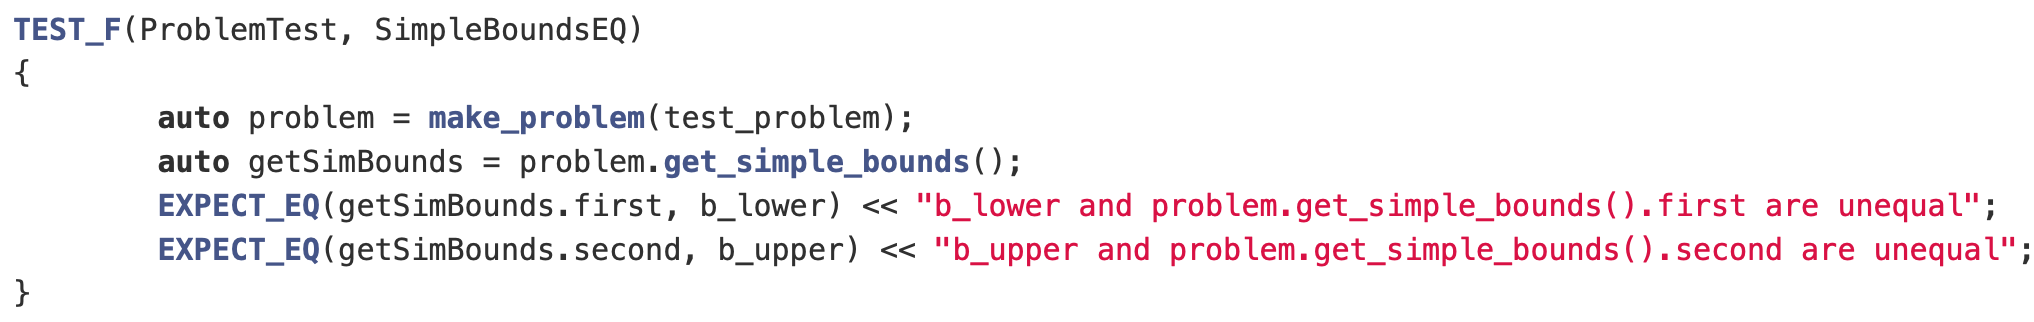
\includegraphics[width=0.9\textwidth]{test1.1.png}
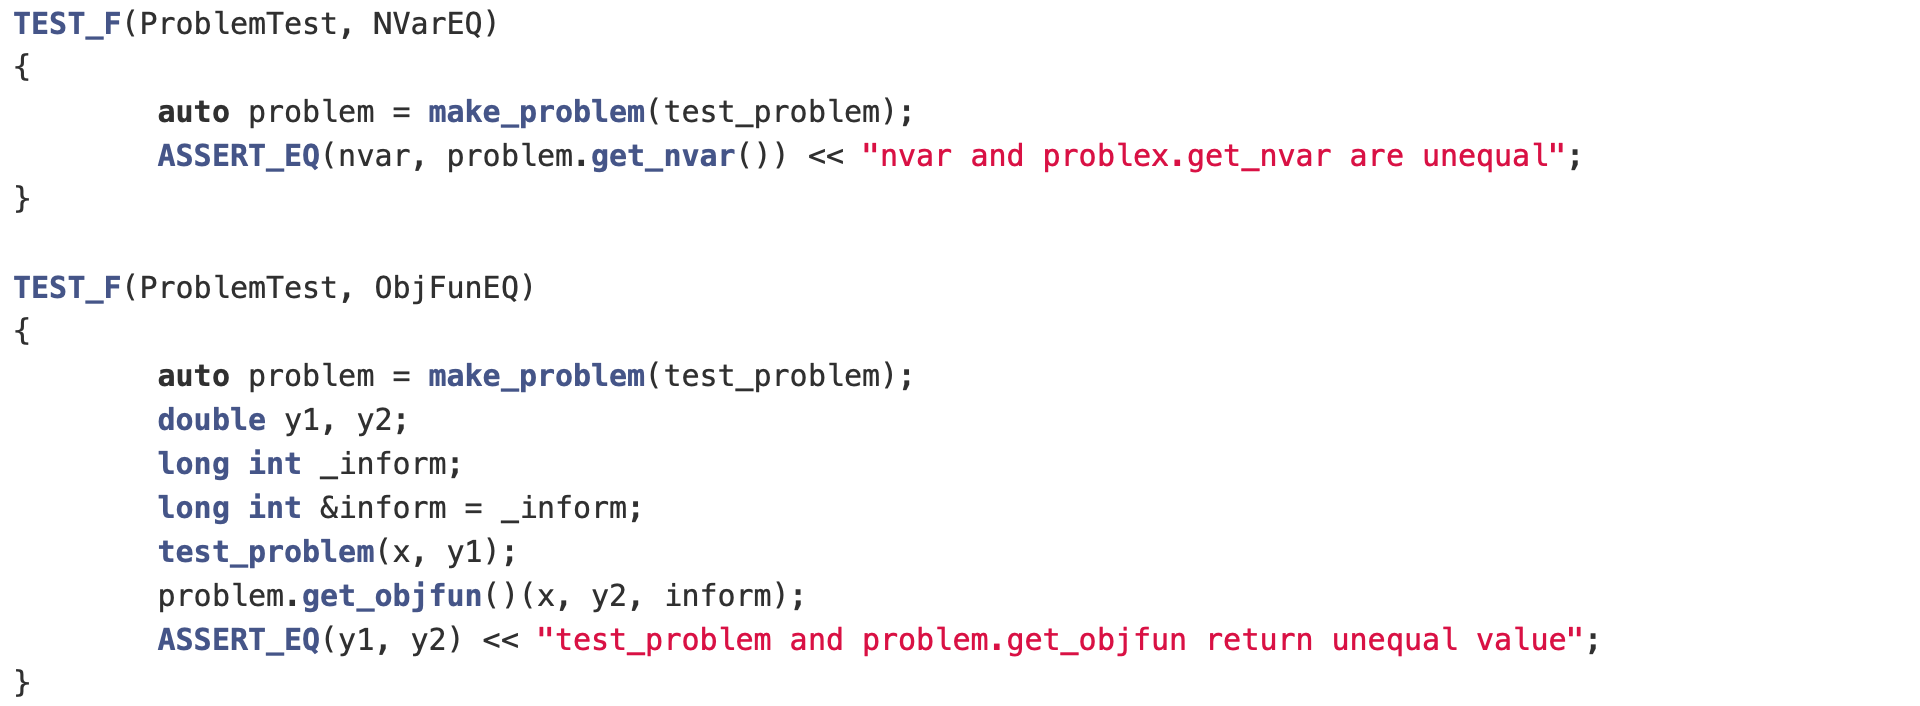
\includegraphics[width=0.9\textwidth]{test1.2.png}
\end{frame}

\begin{frame}
\frametitle{Implementation \\
\small \color{rwth-blue} Software Tests}
\vspace{1em}
\textit{2. Derivatives computation (test\_dco.cpp):}\vspace{1em}
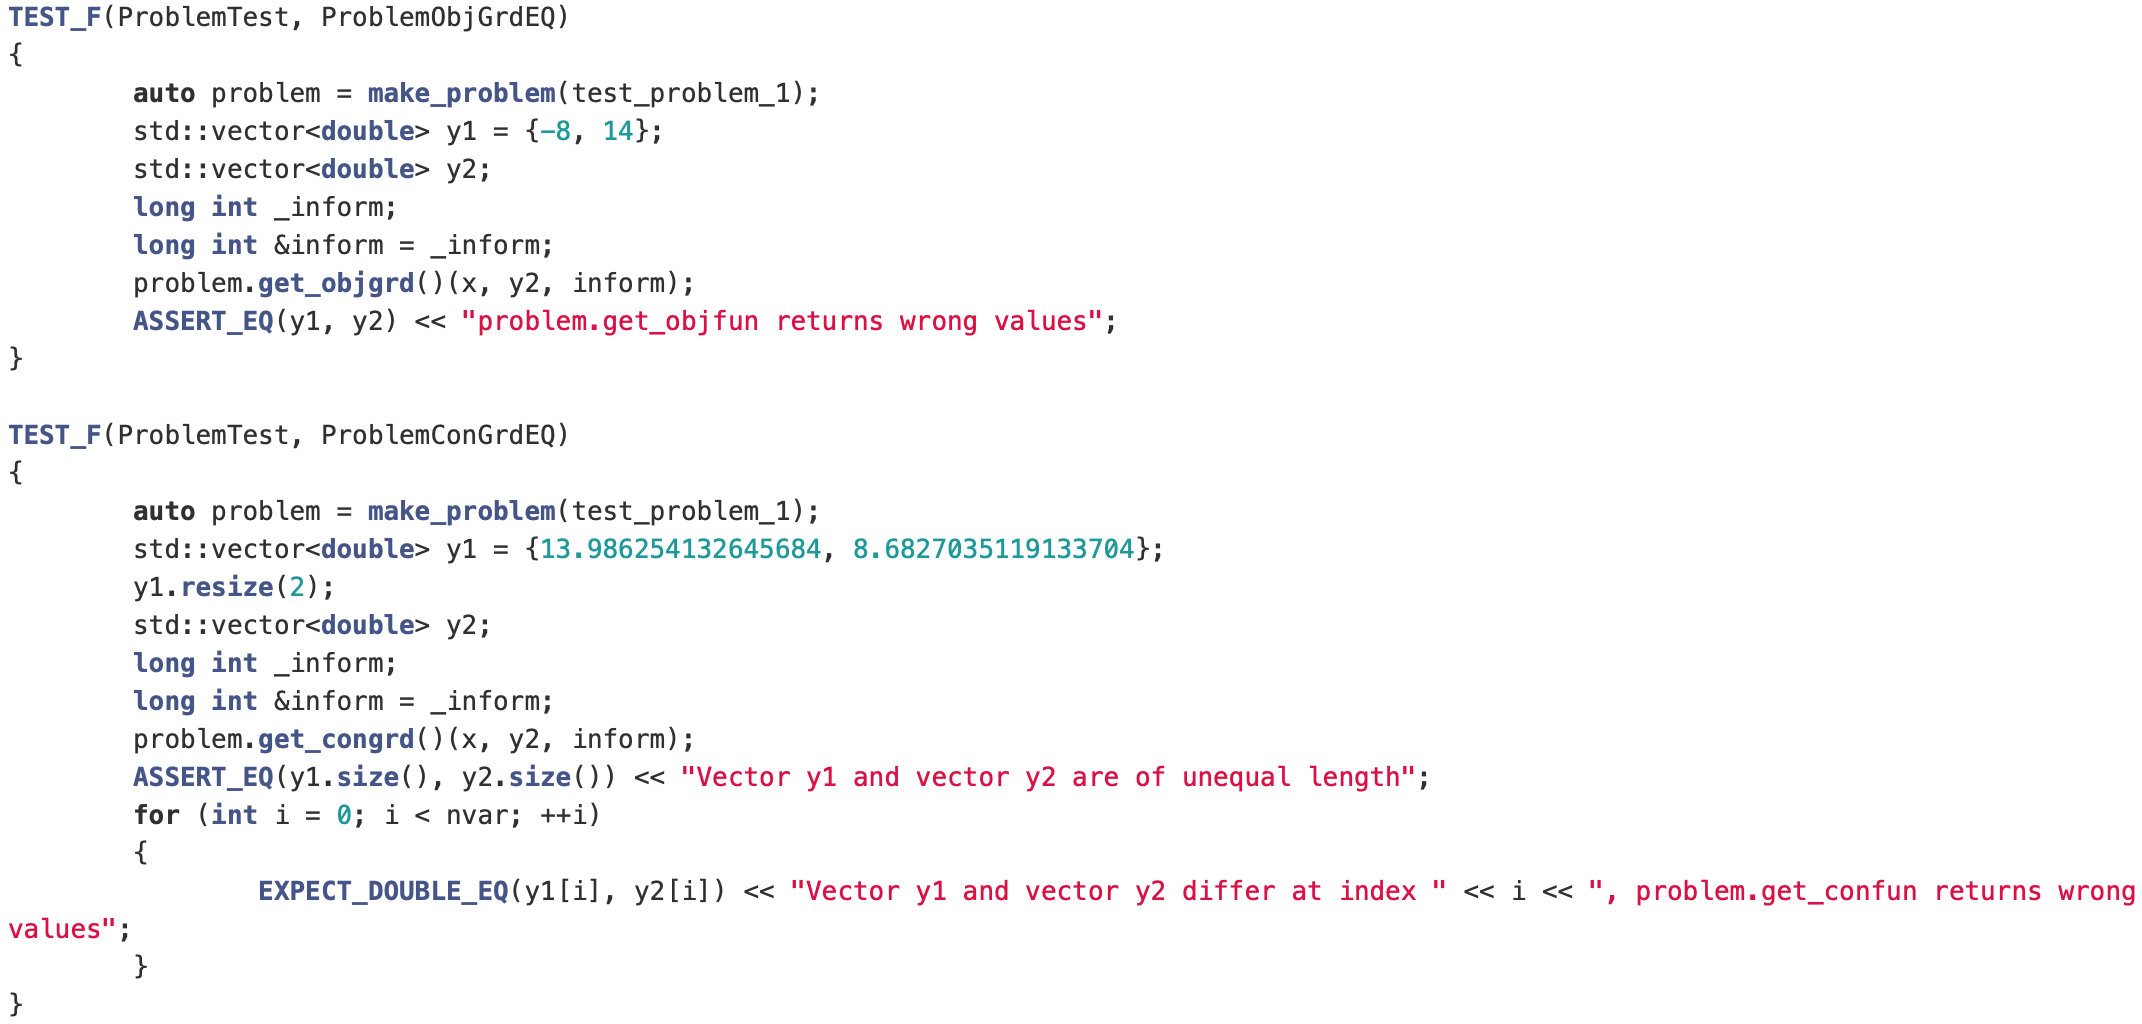
\includegraphics[width=\textwidth]{test2.png}
\end{frame}

\begin{frame}
\frametitle{Implementation \\
\small \color{rwth-blue} Software Tests}
\vspace{1em}
\textit{3. More complex linearity detection logic (test\_linearity.cpp):}\vspace{1ex}

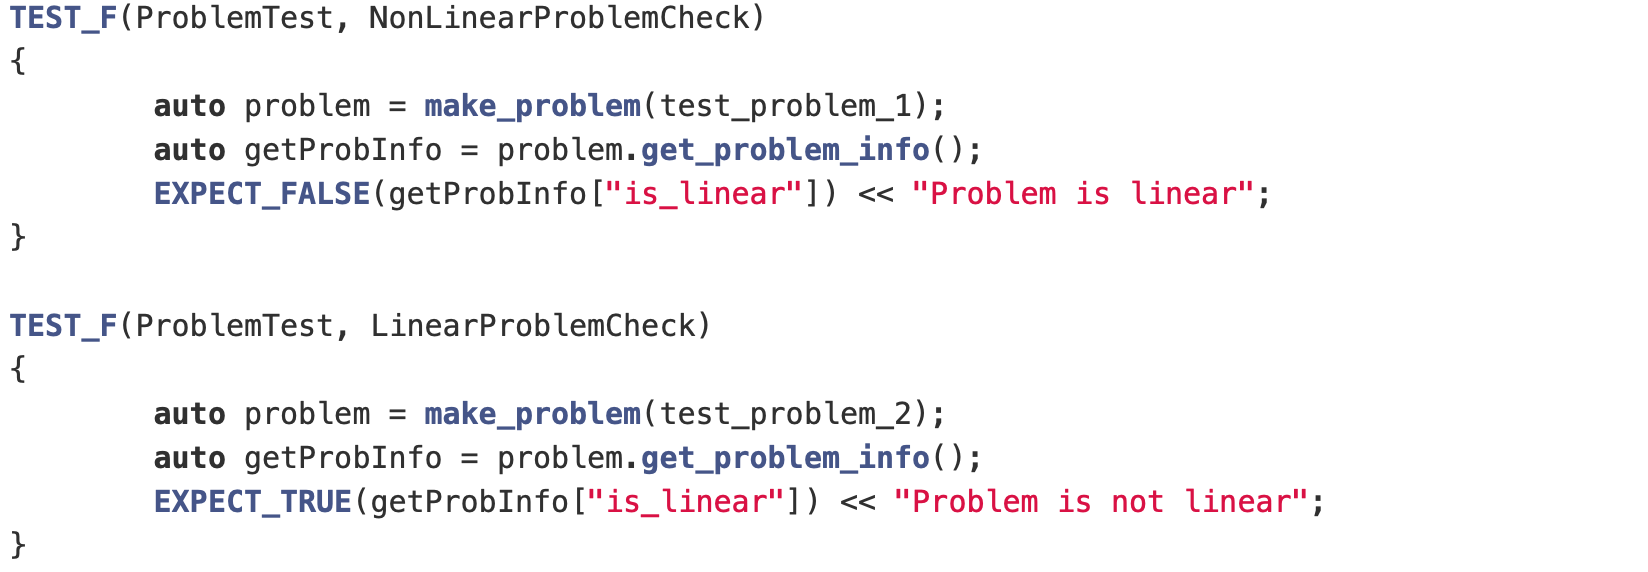
\includegraphics[width=0.7\textwidth]{test3.1.png}
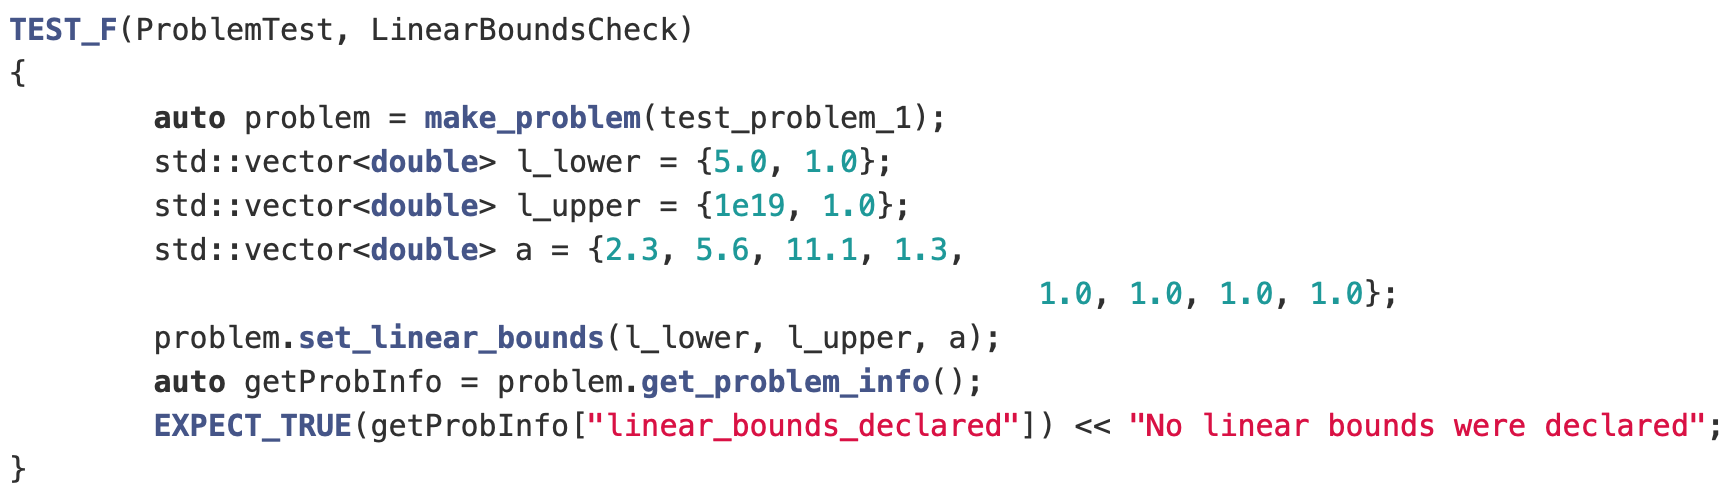
\includegraphics[width=0.7\textwidth]{test3.2.png}
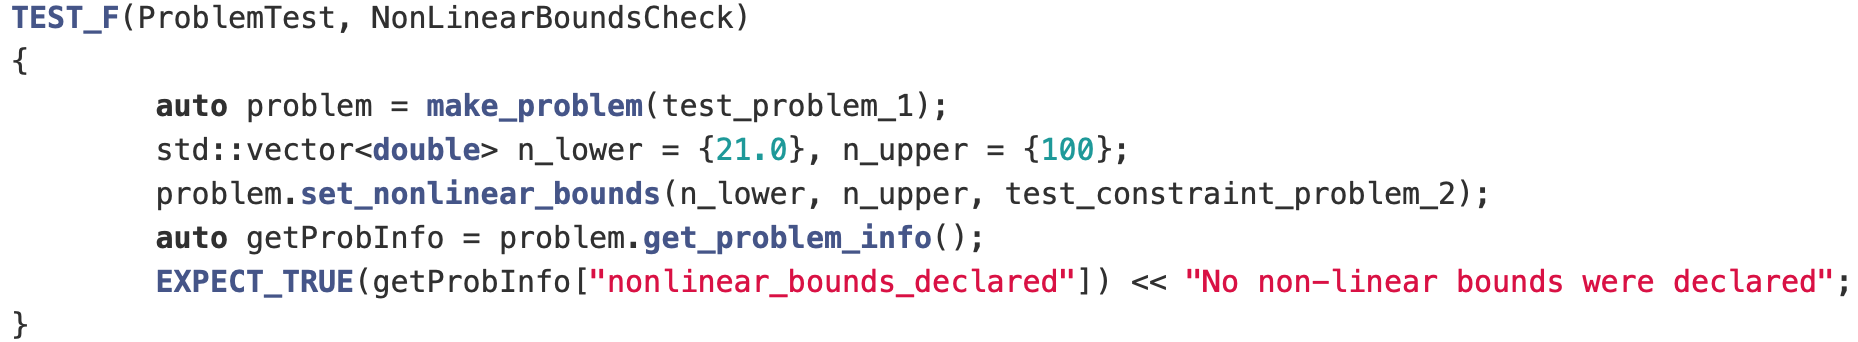
\includegraphics[width=0.7\textwidth]{test3.3.png}
\end{frame}

\subsection{Software Examples}
\begin{frame}
\frametitle{Implementation \\
\small \color{rwth-blue} Software Examples}
\textbf{e04kf solver:}\\
\centering
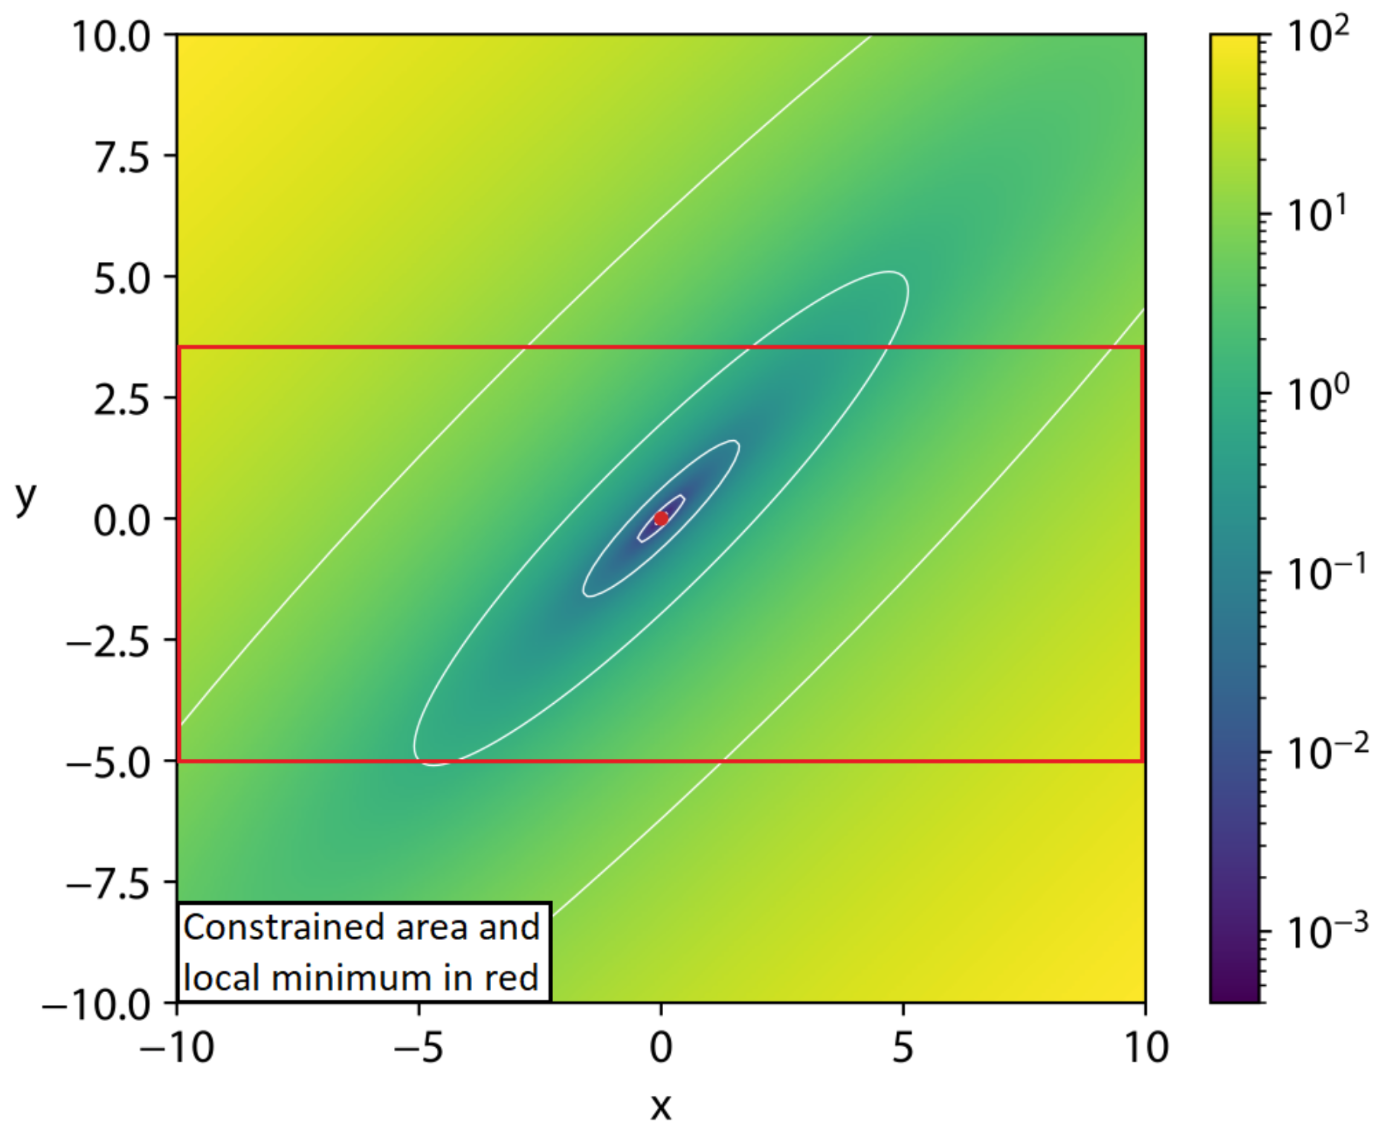
\includegraphics[width=0.5\textwidth]{eg_kf.png}\\
(Matyas function)$^{[1]}$ \\$\mathbb{R}^2\rightarrow \mathbb{R}$, $f(x)=0.26({x}^2+{y}^2)-0.48{x}{y}$\\
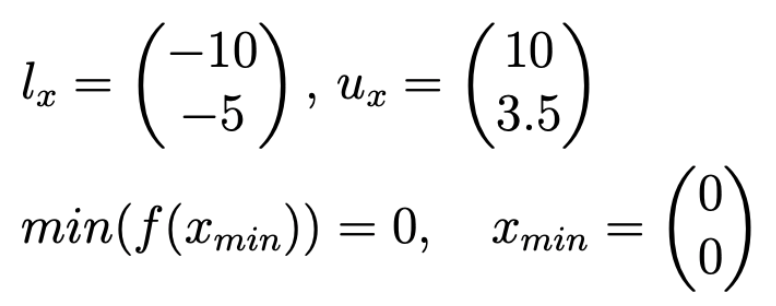
\includegraphics[width=0.4\textwidth]{eg_kf2.png}
\end{frame}

\begin{frame}
\frametitle{Implementation \\
\small \color{rwth-blue} Software Examples}
\textbf{e04mt solver:}\\
\centering
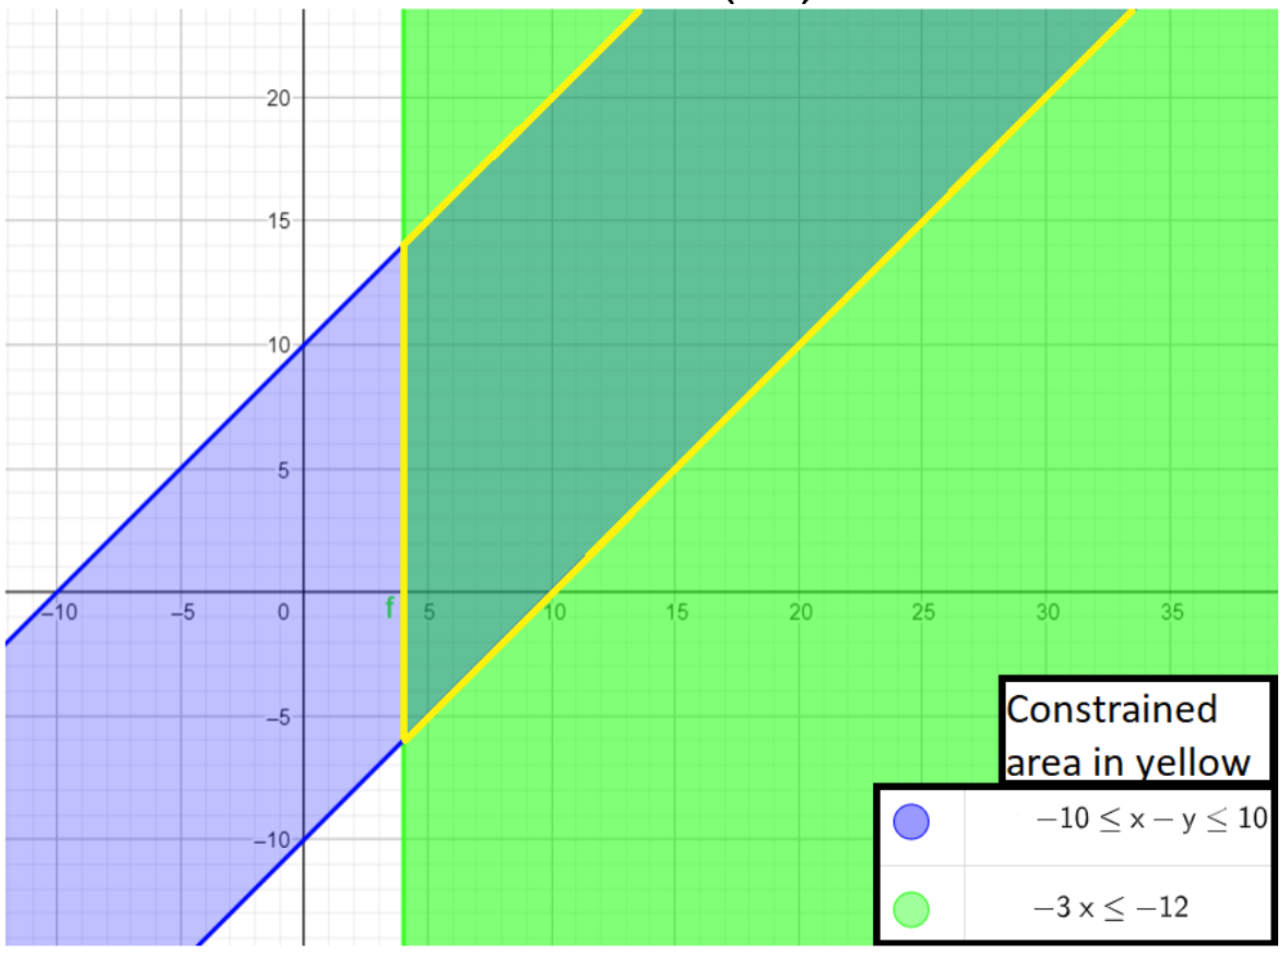
\includegraphics[width=0.5\textwidth]{eg_mt.png}\tiny{[2]}
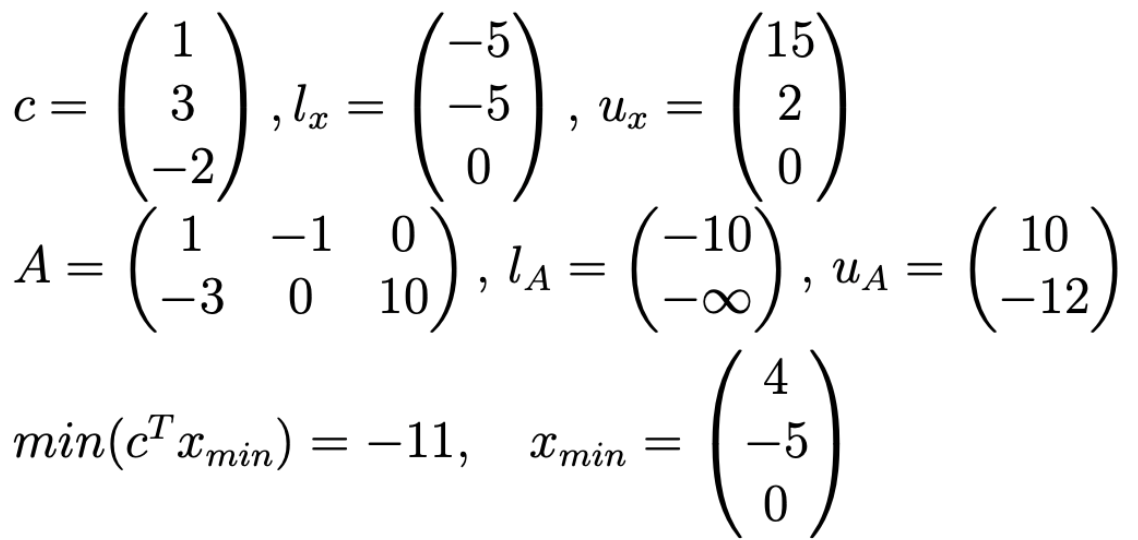
\includegraphics[width=0.5\textwidth]{eg_mt2.png}
\end{frame}

\begin{frame}
\frametitle{Implementation \\
\small \color{rwth-blue} Software Examples}
\textbf{e04st solver:}\\
\centering
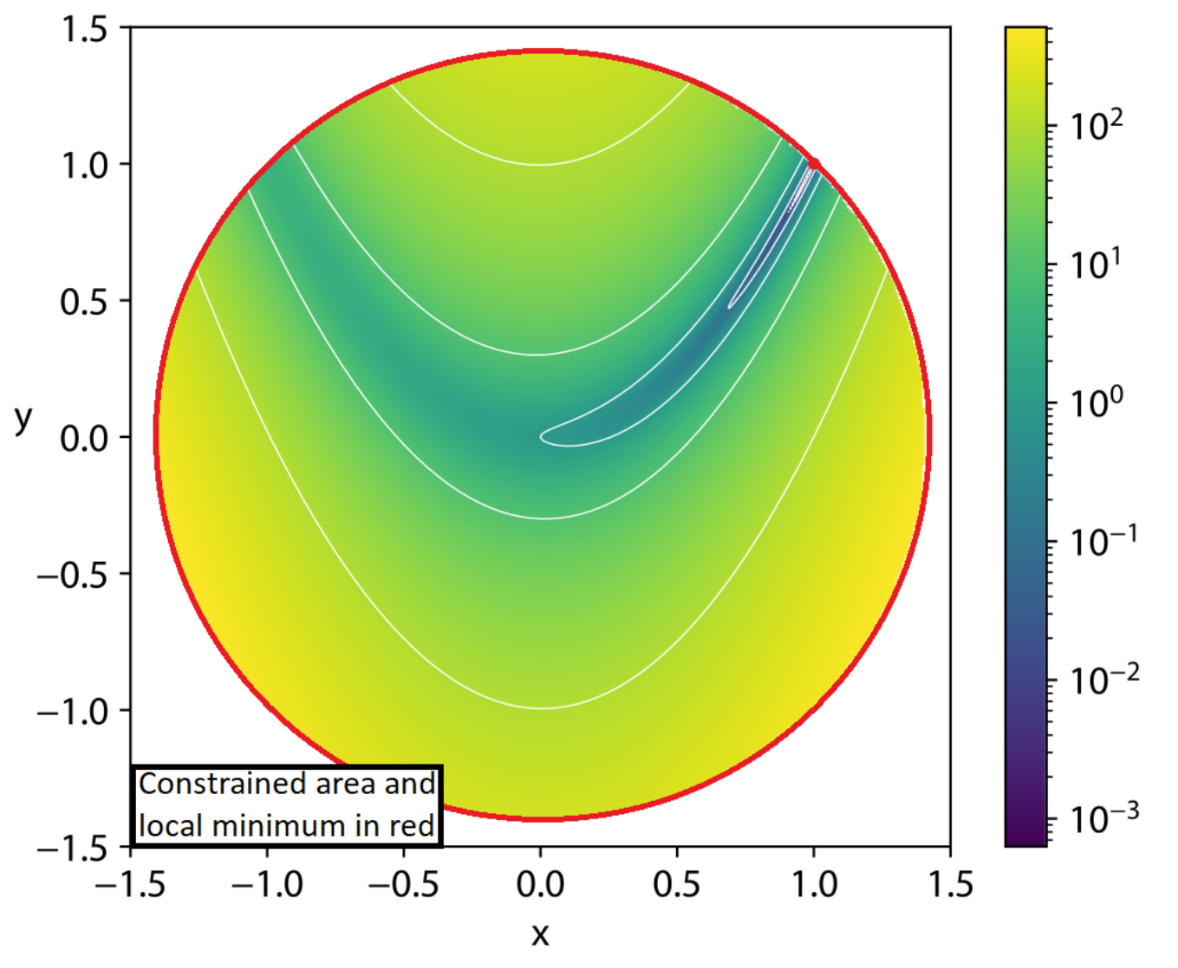
\includegraphics[width=0.4\textwidth]{eg_st.png}\\
\small{(Rosenbrock on disk) $^{[1]}$\\$f(x)=(1-{x})^2+100\cdot ({y}-{x}^2)^2$}\\
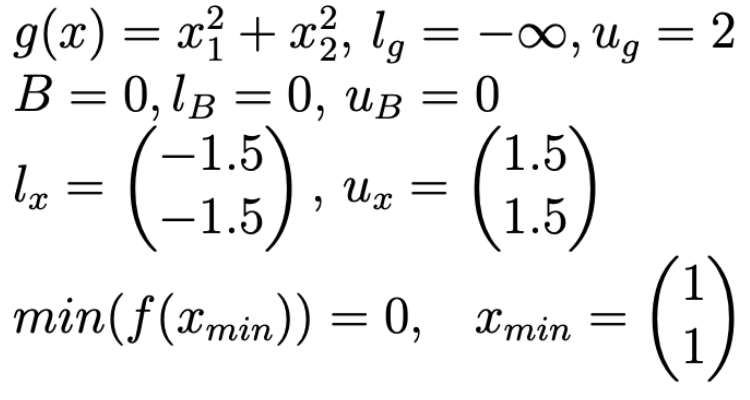
\includegraphics[width=35ex]{eg_st2.png}
\end{frame}

\section{Live Software Demo}
\begin{frame}
\frametitle{Live Software Demo} 
\begin{itemize}
	\item make a build folder \texttt{mkdir build \&\& cd build}
	\item run \texttt{cmake \$\{REPO\_DIR\} -DNAG\_dco\_cpp\_DIR=\$\{HOME\}/NAG/dcl6i37ngl\_v370/ -DNAG\_Library\_DIR=\$\{HOME\}/NAG/nll6i285bl/}
	\item run \texttt{make caseStudies.xxx}
	\item run \texttt{./caseStudies/caseStudies.xxx}
	\item Inspect output
	\item Modify in \texttt{caseStudies/xxx/*.cpp}
\begin{itemize}
	\item objective functions
	\item constraint functions
	\item bounds
	\item solver printing parameters
	\item automatic switch by changing \texttt{con\_function} from non-linear to linear
\end{itemize}
\end{itemize}
\end{frame}


\section{Project Management}

\begin{frame}
\frametitle{Project Management}
\vspace{1ex}
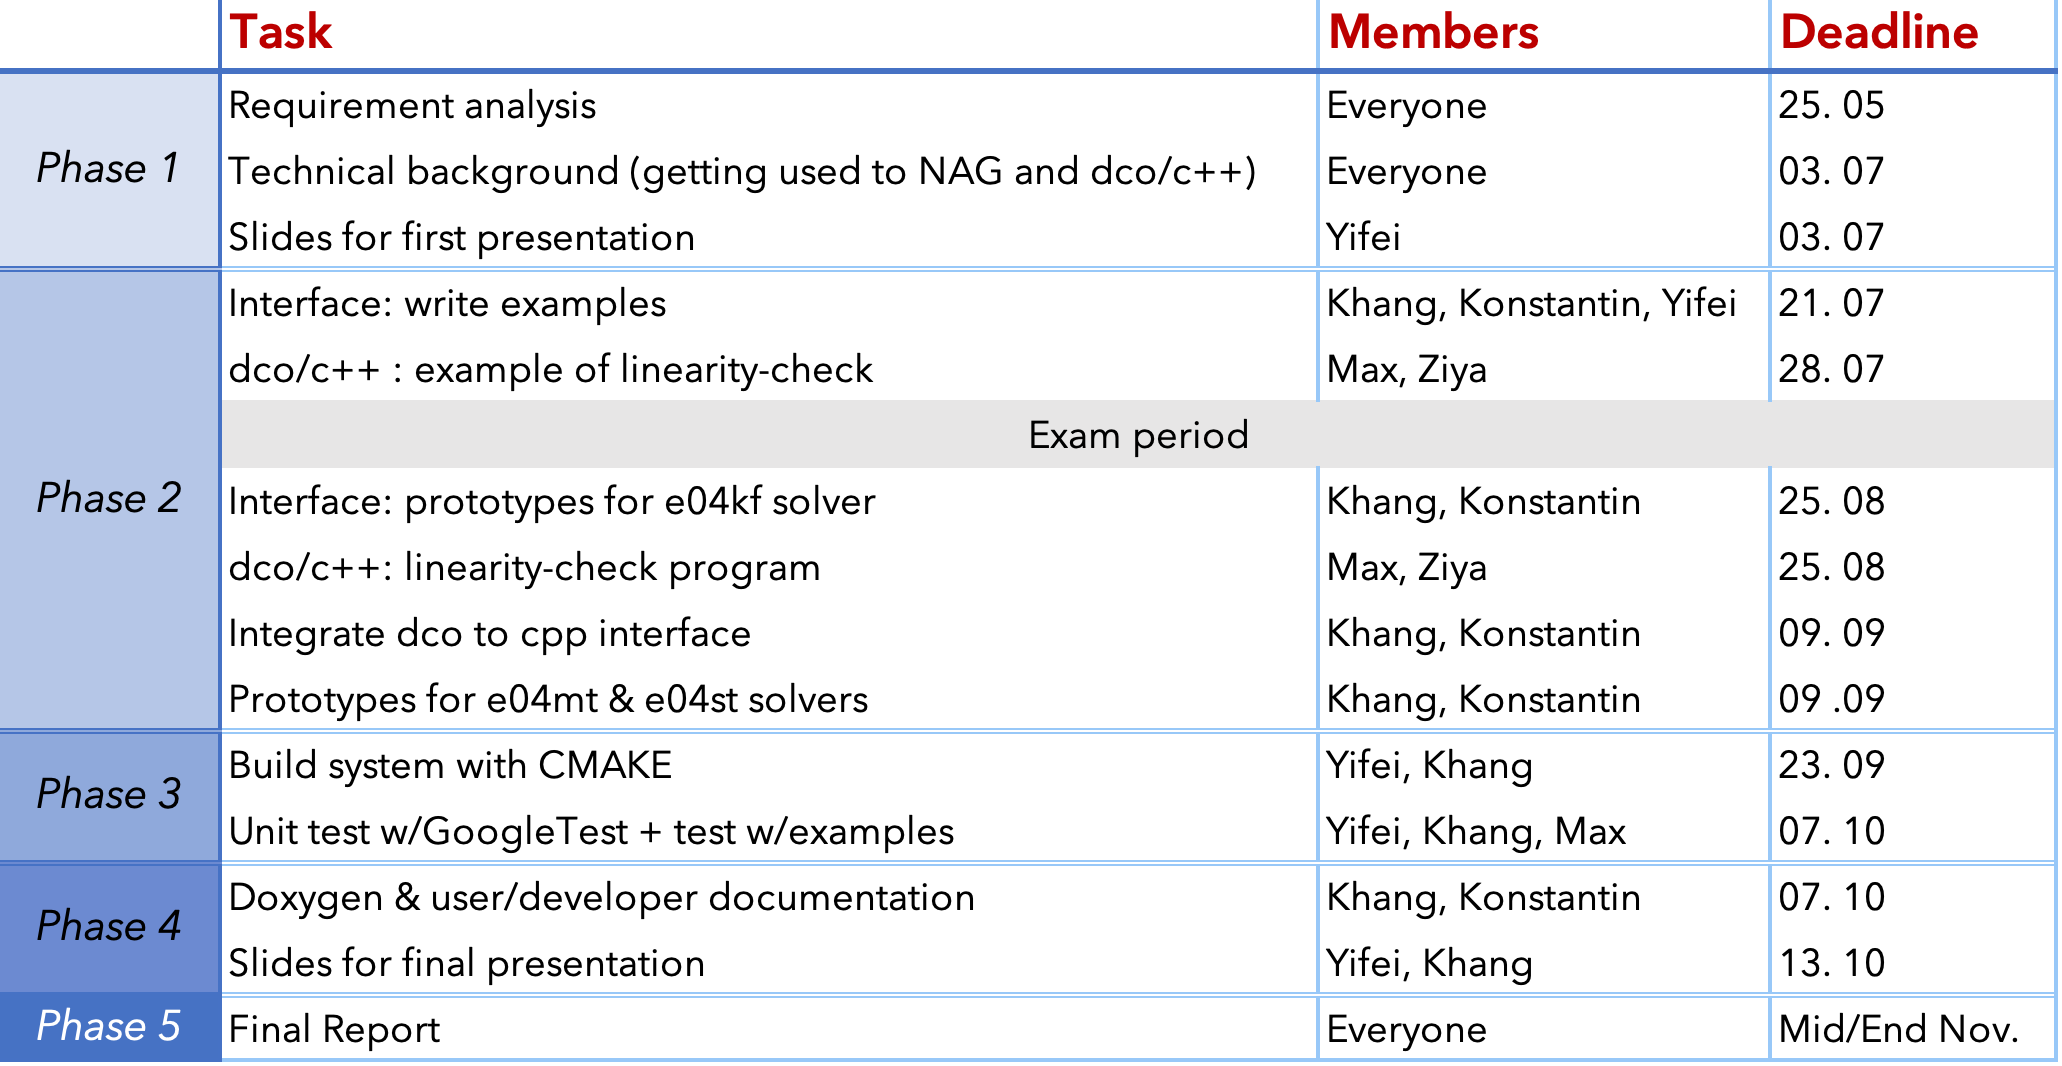
\includegraphics[width=0.9\textwidth]{proj_management.png}
\begin{itemize}
	\item Group meetings every week to discuss work.
	\item Group meetings with supervisor every 2 week to have them check on progress.
	\item Tasks were always assigned to pair, if one person is unavailable there is still another, which proved much of use.
\end{itemize}
\end{frame}


\section{Summary and Conclusion}
\begin{frame}
\frametitle{Summary and Conclusion}
\begin{itemize}
	\item We successfully developed a new object oriented C++ UI for NAG optimization modelling suite (NOMS) using the NAG library and dco/c++ for Automatic Diffrentiation that allows users to define and solve various optimization problems in a uniform manner. 
	\item Our C++ interface is able to separate the definition of the optimization problem and the call to the solver so that it is possible to set up a problem in the same way for different solvers. 
	\item We found at least three examples for each solver which are used in testing for the interface.
	\item We worked as a group, kept our communication both internal and with our supervisor Johannes, managed the time and overcame exceptional situations such as sickness, which was precious experience in software development for all of us. 
\end{itemize}
\end{frame}

\begin{frame}
\frametitle{Reference}
\begin{enumerate}
	\item image source: https://en.wikipedia.org/wiki/Test\_functions\_for\_optimization  
	\item image made with desmos.com 
	\item NAG-Library manual: https://www.nag.com/numeric/nl/nagdoc\_latest/nlhtml/\\ -frontmatter/manconts.html
\end{enumerate}
\end{frame}

\begin{frame}
\LARGE\textbf{Thank you for listening!}
\end{frame}
\end{document}
